\chapter{深度里兹法求解拟线性偏微分方程}
% \section{预备知识与记号}\label{sec:pre}
% 在本文中，我们考虑如下半线性椭圆方程：
% \begin{equation}\label{eq:maineq}
% \left\{\begin{aligned}
% -\Delta u+f(u) &=g & & \text { in } \Omega \\
%  u + \frac{1}{\varepsilon}\frac{\partial u}{\partial n} &=h & & \text { on } \partial \Omega
% \end{aligned}\right.
% \end{equation}
% 其中 $\varepsilon\in (0,+\infty]$。$\varepsilon$ 的区间包含了 Dirichlet 边界条件 ($\varepsilon=+\infty$) 和 Robin 边界条件 ($\varepsilon\in (0,+\infty)$) 的情形。
% 我们对方程施加如下限制：

% \begin{remark}\label{ass:f}
% \begin{itemize}
% \item $\Omega\subset \mathbb{R}^{d}$ 是有界且光滑的。
% \item 对于某个常数 $C$，满足 $|f(x)|\leq C\left(|x|+1\right)^{\frac{d}{d-2}}$。$f$ 是 Lipschitz 连续且单调递增的。
% \item 对于某个 $p\geq 2$，有 $g\in L^{p}$。
% \item 在 $\Omega^{'}\supset \bar{\Omega}$ 上存在一个调和函数 $w$，使得
% $
% w+\frac{1}{\varepsilon}\frac{\partial w}{\partial n}=h
% $
% 在 $\partial \Omega$ 上成立。
% \end{itemize}

% 我们记 $F$ 为 $f$ 的原函数，因此 $F$ 是一个凸函数。
% \end{remark}

% 根据 Schauder 理论可得：

% \begin{theorem}
% 在假设 \ref{ass:f} 下，可知存在且唯一存在一个 $u^{\varepsilon} \in W^{2,2}(\Omega)$ 作为方程~\eqref{eq:maineq} 的解，且 $\|u^{\varepsilon}\|_{W^{2,2}}$ 可被 $g$ 和 $h$ 控制。
% \end{theorem}
% \begin{proof}
% 参见 \cite{2013Roubiek} 中的命题 2.104。
% \end{proof}

% 接下来，介绍我们所使用的神经网络及其记号。深度神经网络 $u_{\phi}:\mathbb{R}^{d}\rightarrow\mathbb{R}$ 定义为
% \begin{equation*}
% \begin{aligned}
% &u_{0}(\boldsymbol{x})=\boldsymbol{x} \\
% &u_{\ell}(\boldsymbol{x})=\sigma_{\ell}\left(A_{\ell} u_{\ell-1}+b_{\ell}\right), \quad \ell=1,2, \ldots, L-1 \\
% &u=u_{L}(\boldsymbol{x})=A_{L} u_{L-1}+b_{L}
% \end{aligned}
% \end{equation*}
% 其中 $A_{\ell}\in\mathbb{R}^{N_{\ell}\times N_{\ell-1}}$, $b_{\ell}\in\mathbb{R}^{N_{\ell}}$，且 $\sigma_{\ell}$ 表示第 $\ell$ 层的激活函数。神经网络 $u_{\phi}$ 的深度 $\mathcal{D}$ 和宽度 $\mathcal{W}$ 定义为
% \begin{equation*}
% \mathcal{D}=L, \ \mathcal{W}=\max\{N_{\ell}:\ell=1,2,\ldots,L\}.
% \end{equation*}
% $\sum_{\ell=1}^{L}N_{\ell}$ 称为 $u_{\phi}$ 的单元数，而 $\phi=\{A_{\ell},b_{\ell}\}_{\ell=1}^{N}$ 称为网络的自由参数。
% \begin{definition}
% 类 $\mathcal{N}^{\alpha}(\mathcal{D},\mathcal{W},\mathcal{B})$ 是满足以下条件的神经网络 $u_{\phi}$ 的集合：
% \begin{itemize}
% \item[(i)] 深度和宽度分别为 $\mathcal{D}$ 和 $\mathcal{W}$；
% \item[(ii)] $u_{\phi}(\boldsymbol{x})$ 的函数值及其导数 $\nabla u_{\phi}(\boldsymbol{x})$ 被 $\mathcal{B}$ 有界控制；
% \item[(iii)] 激活函数由 $\mathrm{ReLU}^{\alpha}$ 给出，其中 $\alpha$ 是一个（多重）指标。
% \end{itemize}
% \end{definition}
% 例如，$\mathcal{N}^{2}(\mathcal{D},\mathcal{W},\mathcal{B})$ 是激活函数为 $\mathrm{ReLU}^2$ 的网络类，而 $\mathcal{N}^{1,2}(\mathcal{D},\mathcal{W},\mathcal{B})$ 是激活函数为 $\mathrm{ReLU}^1$ 或 $\mathrm{ReLU}^2$ 的网络类。若无歧义，我们可以简单地使用 $\mathcal{N}^\alpha$。

% \section{模型构建}\label{sec:mod}

% \begin{theorem}\label{thm:model}
% 对于 $v\in H^{1}(\Omega)$，令
% \begin{equation}\label{eq:conloss}
% \mathcal{L}^{\varepsilon}(v) = \int_{\Omega} \|\nabla v\|_{2}^{2} + 2F(v) - 2vg\,dx + \varepsilon \int_{\partial \Omega}v^{2} - 2vh\,ds.
% \end{equation}
% 则
% \begin{itemize}
% \item 对于 $\varepsilon\in (0,+\infty)$，$\mathcal{L}^{\varepsilon}$ 存在唯一的极小值点，记为 $u^{\varepsilon}$。它是方程 Eq.~\eqref{eq:maineq} 的解。
% \item 当 $\varepsilon \rightarrow +\infty$ 时，设 $u^{\infty}$ 为具有 Dirichlet 边界条件的方程 Eq.~\eqref{eq:maineq} 的解。则我们有：

% \textcolor{black}{\begin{equation*}
% \|u^{\varepsilon}-u^{\infty}\|_{H^{1}}\leq C(\Omega,f,g,h)\frac{1}{\varepsilon}.
% \end{equation*}}

% \end{itemize}
% \end{theorem}
% \begin{proof}
% 如果 $\varepsilon<+\infty$，Eq.~\eqref{eq:conloss} 的欧拉-拉格朗日方程可写为：
% \begin{equation*}
% \begin{array}{rcl}
% \delta \mathcal{L}^{\varepsilon}(v)&=&\displaystyle 2\int_{\Omega}\nabla v^{T}\nabla \delta v + f(v) \delta v - g\delta v\,dx + 2\varepsilon\int_{\partial \Omega}(v-h)\delta v\,ds\\
% {}&=&\displaystyle 2\int_{\Omega} \left(-\Delta v+f(v)-g\right)\delta v\,dx + 2\varepsilon\int_{\partial \Omega} \left(v+\frac{1}{\varepsilon}\frac{\partial v}{\partial n}-h\right) \delta v\,ds.\\
% \end{array}
% \end{equation*}

% Eq.~\eqref{eq:conloss} 的所有临界点必须是 Eq.~\eqref{eq:maineq} 的解，反之亦然。因此，存在唯一的临界点。此外，Eq.~\eqref{eq:conloss} 的凸性保证了该临界点即为极小值点。

% 考虑到 Dirichlet 边界条件，我们将 $w^{\varepsilon}$ 设置为满足以下方程的解：
% \begin{equation*}
% \left\{\begin{aligned}
% -\Delta w^{\varepsilon} +f(u^{\infty})&=g \quad \text { 在 } \Omega \text{ 中} \\
%  w^{\varepsilon}+\frac{1}{\varepsilon}\frac{\partial w^{\varepsilon}}{\partial n} &=h \quad \text { 在 } \partial \Omega \text{ 上},
% \end{aligned}\right.
% \end{equation*}
% 已知（参见 \cite{Maury2009Numerical}（命题 2.3 的证明））：
% $\|w^{\varepsilon}-u^{\infty}\|_{H^{1}}\leq C(\Omega,f(u^{\infty}),g,h)\frac{1}{\varepsilon}$。
% 经典的线性椭圆理论为我们提供了：
% \begin{equation*}
% \int_{\Omega}\|\nabla (w^{\varepsilon}-u^{\varepsilon})\|_{2}^{2}\,dx + \varepsilon \int_{\partial \Omega}(w^{\varepsilon}-u^{\varepsilon})^{2}\,ds \leq \|f(u^{\infty})-f(u^{\varepsilon})\|^{2}_{H^{-1}}\leq C(\Omega,f,u^{\infty}),
% \end{equation*}
% 给定 $f(u^{\varepsilon}),f(u^{\infty})\in L^{2}$。
% 则 $\{u^{\varepsilon}\}$ 是 $H^{1}$ 中的有界序列。但是
% \begin{equation}\label{eq:seminormcontrol}
% \begin{array}{rcl}
% \displaystyle\int_{\Omega}\|\nabla(u^{\infty}-u^{\varepsilon})\|_{2}^{2}\,dx&=&\displaystyle\int_{\Omega}\nabla (u^{\infty}-u^{\varepsilon})^{T}\nabla u^{\infty}\,dx-\int_{\Omega}\nabla (u^{\infty}-u^{\varepsilon})^{T}\nabla u^{\varepsilon}\,dx\\
% {}&{}&{}\\
% {}&=&\displaystyle\int_{\Omega}-\left(u^{\infty}-u^{\varepsilon}\right)\Delta u^{\infty}\,dx-\int-\left( u^{\infty}-u^{\varepsilon}\right)\Delta u^{\varepsilon}\,dx +\\
% {}&{}&\displaystyle\int_{\partial \Omega}\frac{\partial u^{\infty}}{\partial n}(u^{\infty}-u^{\varepsilon})\,ds-\int_{\partial \Omega}\frac{\partial u^{\varepsilon}}{\partial n}(u^{\infty}-u^{\varepsilon})\,ds\\
% {}&{}&{}\\
% {}&=&\displaystyle-\int_{\Omega} \left[f(u^{\infty})-f(u^{\varepsilon})\right]\left(u^{\infty}-u^{\varepsilon}\right)\,dx \\
% {}&{}&\displaystyle+\frac{1}{\varepsilon} \int_{\partial \Omega}\frac{\partial u^{\infty}}{\partial n}\frac{\partial u^{\varepsilon}}{\partial n}\,ds-\frac{1}{\varepsilon} \int_{\partial \Omega}\left(\frac{\partial u^{\varepsilon}}{\partial n}\right)^{2}\,ds\\
% {}&{}&{}\\
% {}&\leq&\displaystyle\frac{1}{2\varepsilon}\left[\int_{\partial \Omega}\left(\frac{\partial u^{\infty}}{\partial n}\right)^{2}-\left(\frac{\partial u^{\varepsilon}}{\partial n}\right)^{2}\,ds\right]\leq C(\Omega,f,g,h)\frac{1}{\varepsilon},
% \end{array}
% \end{equation}
% 注意到 $f$ 是非递减的。
% 接下来，我们将 $u^{\infty}$ 代入 $\mathcal{L}^{\varepsilon}$，得到：
% \begin{equation*}
% \mathcal{L}^{\varepsilon}(u^{\varepsilon})\leq \mathcal{L}^{\varepsilon}(u^{\infty}) \leq C(\Omega,f,g,h) - \varepsilon\int_{\partial \Omega}h^{2}。
% \end{equation*}
% 因此
% \begin{equation*}
% \varepsilon\int_{\partial \Omega}(u^{\varepsilon}-h)^{2}\leq C(\Omega,f,g,h)。
% \end{equation*}
% 结合等式~\eqref{eq:seminormcontrol}，我们可以推导出所需的结论。

% \end{proof}

% 转到 DRM 的第二步，我们将试探函数替换为神经网络：
% \begin{equation*}
% u^{\varepsilon}_{\phi}\in \underset{v \in \mathcal{N}^{2}}{\operatorname{argmin}}\,\mathcal{L}^{\varepsilon}(v),
% \end{equation*}
% 损失函数的离散形式表示如下\cite{chen2021quasi}：
% \begin{equation}\label{eq:disloss}
% \begin{aligned}
% \widehat{\mathcal{L}}_{K}^{\varepsilon}(v) = & \frac{|\Omega|}{N}\sum\limits_{i=1}^{N} \left[ \|\nabla v(X_{i})\|_{2}^{2}+2F\left(v(X_{i})\right)-2g_{K}(X_{i})v(X_{i})\right]\\
% &+\varepsilon\frac{|\partial\Omega|}{M}\sum\limits_{j=1}^{M}\left[v^{2}(Y_{j})-2v(Y_{j})h(Y_{j})\right],
% \end{aligned}
% \end{equation}
% 其中 $\{X_{k}\}_{k=1}^{N}\sim U(\Omega)$ 独立同分布，$\{Y_{j}\}_{j=1}^{M}\sim U(\partial\Omega)$ 独立同分布，且 $g_{K} = \min\{g,K\}$，$K$ 为某个常数。引入截断界 $K$ 是为了避免离散 $\mathcal{L}^{\varepsilon}$ 的不连续性。设 $\widehat{u}^{\varepsilon}_{\phi}$ 为 $\mathcal{N}^{2}$ 上该损失的极小值点：
% \begin{equation}\label{eq:u_hat}
% \widehat{u}^{\varepsilon}_{\phi}\in \underset{v \in \mathcal{N}^{2}}{\operatorname{argmin}}\,\widehat{\mathcal{L}}_{K}^{\varepsilon}(v),
% \end{equation}
% 在随后的讨论中，我们用 $n$ 表示样本数 $N$ 或 $M$。

% \begin{lemma}\label{lemma:energyerr}
% 令 $\widehat{u}^{\varepsilon}_{\phi}$ 为上文定义的函数，我们有：
% \begin{equation*}
% \begin{array}{rcl}
% {}&{}&\mathcal{L}^{\varepsilon}\left(\widehat{u}_{\phi}^{\varepsilon}\right)-\mathcal{L}^{\varepsilon}(u^{\varepsilon})\\
% {}&{}&{}\\
% {}&\leq&\displaystyle\underbrace{ \inf _{u_{\phi} \in \mathcal{N}^{2}}\left[ \mathcal{L}^{\varepsilon}(u_{\phi})- \mathcal{L}^{\varepsilon}(u^{\varepsilon})\right]}_{\mathcal{E}_{\text{app}}}+\underbrace{2 \sup _{u_{\phi} \in \mathcal{N}^{2}}\left|\mathcal{L}^{\varepsilon}_{K}(u_{\phi})-\widehat{\mathcal{L}}^{\varepsilon}_{K}(u_{\phi})\right|}_{\mathcal{E}_{\text{sta}}}+\underbrace{C(g)\mathcal{B}K^{1-p}}_{\mathcal{E}_{\text{tru}}},\\
% \end{array}
% \end{equation*}
% 它们分别被称为逼近误差、统计误差和截断误差。
% \end{lemma}
% \begin{proof}
% 首先，我们介绍一个关于截断误差的简单引理：

% \begin{lemma}\label{lemma:truerr}
% 设 $1\leq q<p<\infty$。如果 $u\in L^{p}$ 且 $u_{N}=u1_{|u|<N}$，则我们有：
% \begin{equation*}
% \|u-u_{N}\|_{L^{q}}\leq C(u)\frac{1}{N^{p/q-1}}.
% \end{equation*}
% \end{lemma}
% \begin{proof}
% 设 $v = |u-u_{N}|$，$f_{v}(t)=m(\{x:v(x)<t\})$，其中 $m$ 是 \textcolor{black}{Lebesgue 测度}。
% \begin{equation*}
% \begin{array}{rcl}
% \|v\|_{L^{q}}^{q}&=&\displaystyle q\int_{0}^{\infty}t^{q-1}f_{v}(t)\,dt\\
% {}&{}&{}\\
% {}&=&\displaystyle q\int_{N}^{\infty}t^{p-1}f_{v}(t)t^{q-p}\,dt\\
% {}&{}&{}\\
% {}&=&\displaystyle qN^{q-p}\int_{N}^{\infty}t^{p-1}f_{v}(t)\,dt\\
% {}&{}&{}\\
% {}&=&\displaystyle qN^{q-p}\|v\|_{L^{p}}^{p}
% \end{array}
% \end{equation*}
% 这便导出了结论。
% \end{proof}
% 令
% \begin{equation*}
% \mathcal{L}_{K}^{\varepsilon}(v)=\int_{\Omega}\|\nabla v\|_{2}^{2}+2 F(v)-2 v g_{K}\,d x+\varepsilon \int_{\partial \Omega} v^{2}-2 v h d s.
% \end{equation*}
% 借助引理 \ref{lemma:truerr}，我们有：
% \begin{equation*}
% |\mathcal{L}_{K}^{\varepsilon}(u_{\phi})-\mathcal{L}^{\varepsilon}(u_{\phi})|\leq\int_{\Omega}|u_{\phi}(g-g_{K})|\,dx\leq C(g)\mathcal{B}K^{1-p},
% \end{equation*}
% 对于任意 $u_{\phi}\in \mathcal{N}^{2}(\mathcal{D},\mathcal{W},\mathcal{B})$。
% 因此，对于任意 $u\in \mathcal{N}^{2}$：
% \begin{equation*}
% \begin{array}{rcl}
% \mathcal{L}^{\varepsilon}\left(\widehat{u}_{\phi}^{\varepsilon}\right)-\mathcal{L}^{\varepsilon}(u^{\varepsilon})&=&\left[\mathcal{L}^{\varepsilon}\left(\widehat{u}_{\phi}^{\varepsilon}\right)-\mathcal{L}_{K}^{\varepsilon}\left(\widehat{u}_{\phi}^{\varepsilon}\right)\right]+\left[\mathcal{L}_{K}^{\varepsilon}\left(\widehat{u}_{\phi}^{\varepsilon}\right)-\widehat{\mathcal{L}}_{K}^{\varepsilon}\left(\widehat{u}_{\phi}^{\varepsilon}\right)\right]\\
% {}&{}&{}\\
% {}&&+\left[\widehat{\mathcal{L}}_{K}^{\varepsilon}\left(\widehat{u}_{\phi}^{\varepsilon}\right)-\widehat{\mathcal{L}}_{K}^{\varepsilon}\left(u_{\phi}\right)\right]+\left[\widehat{\mathcal{L}}_{K}^{\varepsilon}\left(u_{\phi}\right)-\mathcal{L}_{K}^{\varepsilon}\left(u_{\phi}\right)\right]\\
% {}&{}&{}\\
% {}&&+\left[\mathcal{L}_{K}^{\varepsilon}\left(u_{\phi}\right)-\mathcal{L}^{\varepsilon}\left(u_{\phi}\right)\right]+\left[\mathcal{L}^{\varepsilon}\left(u_{\phi}\right)-\mathcal{L}^{\varepsilon}(u^{\varepsilon})\right]\\
% {}&{}&{}\\
% \end{array}
% \end{equation*}
% 该表达式包含六项，其中第一项和第五项表示记为 $\mathcal{E}_{\text{tru}}$ 的真实误差，第二项和第四项对应于记为 $\mathcal{E}_{\text{sta}}$ 的统计误差，第三项为负，而最后一项的下确界恰好等于记为 $\mathcal{E}_{\text{app}}$ 的逼近误差。
% \end{proof}




% \section{主要结果}\label{sec:mainres}
% \subsection{主要定理}
% 针对 Robin 边界条件，我们有：
% \begin{theorem}\label{mainthm:robin}
% 设假设 \ref{ass:f} 成立，且 $\widehat{u}_{\phi}^{\varepsilon}$ 为式 \eqref{eq:u_hat} 中定义的函数。我们有：
% \begin{equation*}
% \|\widehat{u}_{\phi}^{\varepsilon}-u^{\varepsilon}\|_{H^{1}}\leq C(\Omega,u^{\varepsilon},f,g,h)\sqrt{\delta},
% \end{equation*}
% 其中
% \begin{equation*}
% \begin{array}{rcl}
% \delta&\leq&\displaystyle C\left(\Omega, u^{\varepsilon}, f, g, h\right) \varepsilon\left(\mathcal{B}^{-2 / (d-2)}+\mathcal{W}^{-1 / d}\right)+C(g) \mathcal{B}K^{1-p}\\
% {}&{}&{}\\
% {}&{}&\displaystyle+C(\Omega, f, h)(K+\varepsilon \mathcal{B}) \mathcal{B} \mathcal{D}^{2} \mathcal{W} \sqrt{\mathcal{D}+\log \mathcal{W}} \sqrt{\frac{\log n}{n}}.
% \end{array}
% \end{equation*}
% \end{theorem}

% \begin{proof}
% 由引理 \ref{lemma:energyerr} 以及第 \ref{sec:apperr} 节中逼近误差和第 \ref{sec:staerr} 节中统计误差的估计，我们有：
% \begin{equation*}
% \mathcal{L}^{\varepsilon}\left(\widehat{u}_{\phi}^{\varepsilon}\right)-\mathcal{L}^{\varepsilon}\left(u^{\varepsilon}\right)\leq C\left(\Omega, u^{\varepsilon}, f, g, h\right)\delta.
% \end{equation*}
% 令
% \begin{equation*}
% \mathcal{L}^{\varepsilon}_{0}\left(u\right)=\mathcal{L}^{\varepsilon}\left(u\right)-2\int_{\Omega}F(u)\,dx.
% \end{equation*}
% 我们可以推导出：
% \begin{equation*}
% \begin{array}{rcl}
% {}&{}&\displaystyle\mathcal{L}^{\varepsilon}\left(u^{\varepsilon}+v\right)-\mathcal{L}^{\varepsilon}\left(u^{\varepsilon}\right)\\
% {}&{}&{}\\
% {}&=&\displaystyle\mathcal{L}^{\varepsilon}_{0}\left(u^{\varepsilon}+v\right)-\mathcal{L}^{\varepsilon}_{0}\left(u^{\varepsilon}\right) + 2\int_{\Omega}F\left(u^{\varepsilon}+v\right) - F\left(u^{\varepsilon}\right) \,dx\\
% {}&{}&{}\\
% {}&=&\displaystyle\int_{\Omega}\|\nabla \left(u^{\varepsilon}+v\right)\|_{2}^{2}-2 \left(u^{\varepsilon}+ v\right) g\,d x+\varepsilon \int_{\partial \Omega} \left(u^{\varepsilon}+ v\right)^{2}\\
% {}&{}&\displaystyle-2 \left(u^{\varepsilon}+ v\right) h\,d s-\mathcal{L}^{\varepsilon}_{0}\left(u^{\varepsilon}\right)+2\int_{\Omega}f\left(u^{\varepsilon}+\theta v\right)v \,dx\\
% {}&{}&{}\\
% {}&=&\displaystyle\int_{\Omega}\|\nabla v\|_{2}^{2}-2 vg\,d x+\varepsilon \int_{\partial \Omega} v^{2}-2v\left(h-u^{\varepsilon}\right)\, d s\\
% {}&{}&\displaystyle+ 2\int_{\Omega}\nabla v^{T}\nabla u^{\varepsilon}\,dx +2\int_{\Omega}f\left(u^{\varepsilon}+\theta v\right)v \,dx\\
% {}&{}&{}\\
% {}&=&\displaystyle\int_{\Omega}\|\nabla v\|_{2}^{2}d x+\varepsilon \int_{\partial \Omega} v^{2}\, ds+2\int_{\Omega}\left[f\left(u^{\varepsilon}+\theta v\right)-f\left(u^{\varepsilon}\right)\right]v \,dx\\
% {}&{}&{}\\
% {}&\geq &\displaystyle\int_{\Omega}\|\nabla v\|_{2}^{2}\,d x+\varepsilon \int_{\partial \Omega} v^{2}\, d s\gtrsim C(\Omega,\varepsilon)\|v\|_{H^{1}}^{2}, \\
% \end{array}
% \end{equation*}
% 其中 $\theta\in(0,1)$ 是拉格朗日余项的参数。\textcolor{black}{倒数第二个不等式成立基于以下理由：鉴于 $f$ 是单调函数，因此对于任意 $\theta>0$，$f(u^{\varepsilon}+v)-f(u^{\varepsilon})$ 与 $v$ 具有相同的符号，从而使得 $[f(u^{\varepsilon}+v)-f(u^{\varepsilon})]v\geq 0$。}
% \end{proof}

% \begin{corollary}\label{cor:corrobin}
% 在与定理 \ref{mainthm:robin} 相同的条件下，若我们取：
% \begin{equation*}
% \mathcal{D}=O(1),\quad\mathcal{W}=O(n^{t_{1}}),\quad \mathcal{B}=O(n^{t_{2}}),\quad K=O(n^{t_{3}}),
% \end{equation*}
% 我们可以得到：
% \begin{equation*}
% \|\widehat{u}_{\phi}^{\varepsilon}-u^{\varepsilon}\|_{H^{1}}\leq C\left(\Omega, u^{\varepsilon}, f, g, h\right)n^{-t_{4}/2},
% \end{equation*}
% 其中
% \begin{equation*}
% \left\{
% \begin{array}{rcl}
% t_{1}&=&\displaystyle\frac{d(p-1)}{3dp-2d-p+1} \\
% t_{2}&=&\displaystyle\frac{(d-2)(p-1)}{2(3dp-2d-p+1)}\\
% t_{3}&=&\displaystyle\frac{d}{2(3dp-2d-p+1)}\\
% t_{4}&=&\displaystyle\frac{p-1}{3dp-2d-p+1}
% \end{array}
% \right.
% \end{equation*}
% 均为正数。
% \end{corollary}

% 对于 Dirichlet 边界条件，我们有：
% \begin{theorem}\label{mainthm:diri}
% 设假设 \ref{ass:f} 成立，且 $\widehat{u}_{\phi}^{\varepsilon}$ 为等式~\eqref{eq:u_hat} 中定义的函数。我们有：
% \begin{equation*}
% \|\widehat{u}_{\phi}^{\varepsilon}-u^{\infty}\|_{H^{1}}\leq C(\Omega,u^{\varepsilon},f,g,h)\sqrt{\delta},
% \end{equation*}
% 其中
% \begin{equation*}
% \begin{array}{rcl}
% \delta&\leq&C\left(\Omega, u^{\varepsilon}, f, g, h\right) \varepsilon\left(\mathcal{B}^{-2 / (d-2)}+\mathcal{W}^{-1 / d}\right)+C(g) \mathcal{B}K^{1-p}\\
% {}&{}&{}\\
% {}&{}&\displaystyle+C(\Omega, f, h)(K+\varepsilon \mathcal{B}) \mathcal{B} \mathcal{D}^{2} \mathcal{W} \sqrt{\mathcal{D}+\log \mathcal{W}} \sqrt{\frac{\log n}{n}}+C(\Omega,f,g,h)\frac{1}{\varepsilon}.
% \end{array}
% \end{equation*}
% \end{theorem}
% \begin{proof}
% 这是由定理 \ref{mainthm:robin} 和定理 \ref{thm:model} 中的结论直接推导得出的。
% \end{proof}

% \begin{corollary}
% 在定理 \ref{mainthm:diri} 的相同条件下，如果我们取：
% \begin{equation*}
% \varepsilon = O(n^{t_{4}/2}),\quad\mathcal{D}=O(1),\quad\mathcal{W}=O(n^{t_{1}}),\quad \mathcal{B}=O(n^{t_{2}}),\quad K=O(n^{t_{3}}),
% \end{equation*}
% 我们可以得到：
% \begin{equation*}
% \|\widehat{u}_{\phi}^{\varepsilon}-u^{\infty}\|_{H^{1}} \leq C(p)n^{-t_{4}/4},
% \end{equation*}
% 其中 $\{t_{i}\}_{1}^{4}$ 是推论 \ref{cor:corrobin} 中的数值。
% \end{corollary}

% \subsection{逼近误差}\label{sec:apperr}

% \begin{theorem}\label{thm:apperr}

% 如果 $\mathcal{D}$，$\mathcal{W}$ 和 $\mathcal{B}$ 足够大，我们可以建立如下结果：
% \begin{equation*}
% \mathcal{E}_{a p p}=\inf _{u_{\phi} \in \mathcal{N}^{2}(\mathcal{D},\mathcal{W},\mathcal{B})}\left[\mathcal{L}^{\varepsilon}\left(u_{\phi}\right)-\mathcal{L}^{\varepsilon}\left(u^{\varepsilon}\right)\right]\leq C(\Omega,u^{\varepsilon},f)\varepsilon\left(\mathcal{B}^{-2/(d-2)}+\mathcal{W}^{-1/d}\right).
% \end{equation*}
% \end{theorem}

% \begin{proof}
% 我们的证明基于一些经典的多项式逼近结果 \cite{1984Arcangeli}。

% 设 $\rho\in C_{0}^{\infty}$ 为一个磨光器（mollifier）：
% \begin{itemize}
% \item $\int \rho\,dx=1$
% \item $\rho \geq 0$.
% \item 当 $\|x\|> 1$ 时 $\rho(x) = 0$。
% \item $\|\rho(x)\|_{\infty}=2V_{d}$，其中 $V_{d}$ 是单位球的体积。
% \end{itemize}
% 取 $q = \frac{2d}{d-2}$ 并令：
% \begin{equation*}
% u^{\varepsilon}_{\mathcal{B}}(x)=\int_{y}\mathcal{B}^{q}\rho(\frac{y}{\mathcal{B}^{q/d}})u^{\varepsilon}(x+y)\,dy.
% \end{equation*}
% 我们断言：
% \begin{itemize}
% \item $\|u^{\varepsilon}_{\mathcal{B}}\|_{W^{1,\infty}(\Omega)}\leq \left(2V_{d}\|u^{\varepsilon}\|_{W^{2,2}(\Omega)}^{q}+2\right)\mathcal{B}$.
% \item $\|u^{\varepsilon}_{\mathcal{B}}-u^{\varepsilon}\|_{H^{1}(\Omega)}\leq 2\|u^{\varepsilon}\|_{W^{2,2}(\Omega)}\mathcal{B}^{-q/d}.$
% \item $\|u^{\varepsilon}_{\mathcal{B}}\|_{W^{2,2}(\Omega)}\leq \|u^{\varepsilon}\|_{W^{2,2}(\Omega)}$.
% \end{itemize}

% 对于第一个断言，令 $E_{\mathcal{B}}=\{x:|u^{\varepsilon}(x)|>\mathcal{B}\}$，根据引理 \ref{lemma:truerr} 我们有 $\|u^{\varepsilon}1_{E_{\mathcal{B}}}\|_{L^{1}}\leq 2\|u^{\varepsilon}\|_{L^{q}}^{q}\mathcal{B}^{1-q}$。因此：
% \begin{equation*}
% \begin{array}{rcl}
% |u^{\varepsilon}_{\mathcal{B}}(x)|&\leq&\displaystyle\int_{y}\mathcal{B}^{q}\rho(\frac{y}{\mathcal{B}^{q/d}})|u^{\varepsilon}(x+y)|\,dy\\
% {}&{}&{}\\
% {}&=&\displaystyle\int_{E_{\mathcal{B}}}\mathcal{B}^{q}\rho(\frac{y}{\mathcal{B}^{q/d}})|u^{\varepsilon}(x+y)|\,dy+\int_{E_{\mathcal{B}}^{c}}\mathcal{B}^{q}\rho(\frac{y}{\mathcal{B}^{q/d}})|u^{\varepsilon}(x+y)|\,dy\\
% {}&{}&{}\\
% {}&\leq&\displaystyle\|\mathcal{B}^{q}\rho(\frac{y}{\mathcal{B}^{q/d}})\|_{L^{\infty}}\|u^{\varepsilon}1_{E_{\mathcal{B}}}\|_{L^{1}}+\|\mathcal{B}^{q}\rho(\frac{y}{\mathcal{B}^{q/d}})\|_{L^{1}}\|u^{\varepsilon}1_{E_{\mathcal{B}}^{c}}\|_{L^{\infty}}\\
% {}&{}&{}\\
% {}&\leq &\displaystyle\left(2V_{d}\|u^{\varepsilon}\|_{L^{q}}^{q}+1\right)\mathcal{B}.
% \end{array}
% \end{equation*}
% 由于 $\nabla u^{\varepsilon}\in L^{q}$ 且微分算子与磨光器可交换，同样的论证也适用于 $\nabla u^{\varepsilon}_{\mathcal{B}}$。

% 对于第二个断言，我们有：
% \begin{equation*}
% \begin{array}{rcl}
% \displaystyle\|u^{\varepsilon}_{\mathcal{B}}-u^{\varepsilon}\|_{L^{2}}&\leq&\displaystyle\left[\int_{x}\left(\int_{y}\rho(y)\left|u^{\varepsilon}(x+\mathcal{B}^{-q/d}y)-u^{\varepsilon}(x)\right|\,dy\right)^{2}\,dx\right]^{1/2}\\
% {}&{}&{}\\
% {}&\leq&\displaystyle\left[\int_{x}\left(\int_{y}\int_{t=0}^{\mathcal{B}^{-q/d}}\rho(y)\left|y^{T}\nabla u^{\varepsilon}(x+ty)\right|\,dtdy\right)^{2}\,dx\right]^{1/2}\\
% {}&{}&{}\\
% {}&\leq&\displaystyle\left[\int_{x}\left(\int_{y}\int_{t=0}^{\mathcal{B}^{-q/d}}\rho(y)\|y\|_{2}\|\nabla u^{\varepsilon}(x+ty)\|_{2}\,dtdy\right)^{2}\,dx\right]^{1/2}\\
% {}&{}&{}\\
% {}&\leq&\displaystyle\int_{y}\int_{t=0}^{\mathcal{B}^{-q/d}}\left[\int_{x}\rho(y)^{2}\|y\|_{2}^{2}\|\nabla u^{\varepsilon}(x+ty)\|_{2}^{2}\,dx\right]^{1/2}\,dtdy\\
% {}&{}&{}\\
% {}&\leq&\displaystyle\int_{y}\int_{t=0}^{\mathcal{B}^{-q/d}}\rho(y)\|y\|_{2}\|\nabla u^{\varepsilon}(x+ty)\|_{L_{x}^{2}}\,dtdy\\
% {}&{}&{}\\
% {}&=&\displaystyle\|\nabla u^{\varepsilon}\|_{L^{2}}\mathcal{B}^{-q/d},
% \end{array}
% \end{equation*}
% 这对 $\nabla u^{\varepsilon}$ 也成立，因为 $\nabla u^{\varepsilon}\in W^{1,2}$。

% 第三个断言是 Fubini 定理的直接推论。

% 接下来，我们证明 $W^{s,p}(\Omega)$ 中的任意函数都可以在 $W^{1,p}$ 范数下被神经网络 $\tilde{f}$ 逼近，其中 $s>1,\tilde{f}\in\mathcal{N}^{2}$。

% 不失一般性，我们假设 $\Omega\subset [0,1]^{d}$ 并将函数延拓到其中。
% 令
% \begin{equation*}
% \psi(x;\delta) = \frac{2}{\delta^{2}}\left[\mathrm{ReLU}^{2}(x)+\mathrm{ReLU}^{2}(x+\delta)-2\mathrm{ReLU}^{2}(x+\frac{\delta}{2})\right].
% \end{equation*}
% 则 $\psi$ 是一个宽度为 $\{1,3,1\}$ 的 $\mathrm{ReLU}^{2}$-网络，且
% \begin{equation*}
% \psi(x;\delta)=\left\{
% \begin{array}{ll}
% 0&x\in (-\infty, -\delta],\\
% \frac{2}{\delta^{2}}(x+\delta)^{2}&x\in (-\delta, -\frac{\delta}{2}],\\
% -\frac{2}{\delta^{2}}x^{2}+1&x\in (-\frac{\delta}{2},0],\\
% 1&x\in (0,\infty).
% \end{array}
% \right.
% \end{equation*}
% 对于任意多重指标 $\mathbf{I}\in \{1,2,3,\cdots,N\}^{d}$，我们定义
% \begin{equation*}
% \lambda_{\mathbf{I}}(x)=\prod_{j=1}^d\left[\psi\left(x^{(j)}-\frac{\mathbf{I}(j)}{N} ; \frac{1}{N}\right)-\psi\left(x^{(j)}-\frac{\mathbf{I}(j)+1}{N} ; \frac{1}{N}\right)\right]
% \end{equation*}
% 此时 $\lambda_{\mathbf{I}}$ 在 $[0,1]^{d}$ 中构成了单位分解的正部分，且其支集为\\ $U_{\mathbf{I}}=\prod_{j}[\frac{\mathbf{I}(j)-1}{N},\frac{\mathbf{I}(j)+1}{N}]$.
% \textcolor{black}{注意到 $\lambda_{\mathbf{I}}$ 是一个次数至多为 $d$ 的分段多项式函数，并观察到：
% \begin{equation*}
% f(x)g(x)=\frac{1}{4}\left[\mathrm{ReLU}^{2}(f+g)+\mathrm{ReLU}^{2}(-f-g)-\mathrm{ReLU}^{2}(f-g)-\mathrm{ReLU}^{2}(g-f)\right].
% \end{equation*}
% 可以容易推导出 $\lambda_{\mathbf{I}}$ 可以被宽度为 $4d$ 和深度为 $\lceil \log_{2}d\rceil+3$ 的 $\mathrm{ReLU}^{2}$-网络精确表示。}


% \begin{lemma}
% 设 $f\in W^{s,p}(\Omega)\cap W^{1,\infty}(\Omega)$，其中 $s\in (1,2]$。
% 对于任意 $\mathbf{I}$，令\\
% $V_{\mathbf{I}}=\prod_j\left[\frac{I(j)-2}{N}, \frac{I(j)+2}{N}\right]$.
% 则存在一个宽度为 $\{d,\frac{d^{2}+3d+2}{2},1\}$ 的 $\mathrm{ReLU}^{2}$-神经网络 $\Psi_{\mathbf{I}}[f]$，使得
% \begin{itemize}
% \item $\left\|\Psi_{\mathbf{I}}[f]\right\|_{W^{1,\infty}(V_{\mathbf{I}})}\leq 2\|f\|_{W^{1,\infty}(\Omega)}$.
% \item$\|f-\psi_{\mathbf{I}}[f]\|_{W^{1,p}(V_{\mathbf{I}})}\leq C(s,p,d)[f]_{s,p,V_{\mathbf{I}}}N^{1-s},$
% \item$\|f-\psi_{\mathbf{I}}[f]\|_{L^{p}(V_{\mathbf{I}})}\leq C(s,p,d)[f]_{s,p,V_{\mathbf{I}}}N^{-s}.
% $
% \end{itemize}
% \end{lemma}
% \begin{proof}

% 通过审慎地选择 $\{a_{i},b_{i}\}$ 的值，我们可以确保集合 $\{\mathrm{ReLU}^{2}(a_{i}^{T}x+b_{i})\}$ 构成 $P(V_{\mathbf{I}})$ 的一组完备线性基，其中
% \begin{equation*}
% P(V_{\mathbf{I}})=\{V_{\mathbf{I}}\text{ 上所有次数小于 } 2 \text{ 的多项式}\}.
% \end{equation*}
% $P(V_{\mathbf{I}})$ 的维数是 $\frac{d^{2}+3d+2}{2}$。
% 多项式逼近的结果是 \cite{1984Arcangeli} 工作的直接推论。
% \end{proof}

% 现在对于任意 $f\in W^{s,p}(\Omega)$，定义：
% \begin{equation*}
% \tilde{f}=\sum_{\mathbf{I}}\lambda_{\mathbf{I}}\Psi_{\mathbf{I}}[f].
% \end{equation*}
% 由于 $\lambda_{\mathbf{I}}$ 和 $\Psi_{\mathbf{I}}[f]$ 均为 $\mathrm{ReLU}^{2}$-神经网络，由此可知 $\tilde{f}$ 是一个宽度至多为 $N^{d}\left(2d^{2}+6d+2\right)$ 且深度至多为 $\lceil \log_{2}d\rceil+5$ 的神经网络。
% 此外，我们有：
% \begin{equation*}
% \begin{array}{rcl}
% {}&{}&\displaystyle\left\|\partial_{i}f-\partial_{i}\tilde{f} \right\|_{L^{p}(\Omega)}\\
% {}&=&\displaystyle\left\|\partial_{i}\sum\limits_{\mathbf{I}}\lambda_{\mathbf{I}}\left(f-\Psi_{\mathbf{I}}[f]\right)\right\|_{L^{p}(\Omega)}\\
% {}&{}&{}\\
% {}&\leq&\displaystyle\sum\limits_{\mathbf{I}}\left\|\partial_{i}\lambda_{\mathbf{I}}\left(f-\Psi_{\mathbf{I}}[f]\right)\right\|_{L^{p}(\Omega)}+\sum\limits_{\mathbf{I}}\left\|\lambda_{\mathbf{I}}\partial_{i}\left(f-\Psi_{\mathbf{I}}[f]\right)\right\|_{L^{p}(\Omega)}\\
% {}&{}&{}\\
% {}&\leq&\displaystyle\sum\limits_{\mathbf{I}}\left\|\partial_{i}\lambda_{\mathbf{I}}\right\|_{L^{\infty}(V_{\mathbf{I}})}\left\|\left(f-\Psi_{\mathbf{I}}[f]\right)\right\|_{L^{p}(V_{\mathbf{I}})}+\sum\limits_{\mathbf{I}}\left\|\partial_{i}\left(f-\Psi_{\mathbf{I}}[f]\right)\right\|_{L^{p}(V_{\mathbf{I}})}\\
% {}&{}&{}\displaystyle\\
% {}&\leq&\sum\limits_{\mathbf{I}}2NC(s,p,d)[f]_{s,p,V_{\mathbf{I}}}N^{-s}+\sum\limits_{\mathbf{I}}C(s,p,d)[f]_{s,p,V_{\mathbf{I}}}N^{1-s}\\
% {}&{}&{}\\
% {}&\leq&\displaystyle C(s,p,d)[f]_{s,p,\Omega}N^{1-s}.
% \end{array}
% \end{equation*}
% 综上所述，我们现在证明了引理 \ref{lemma:4.7}：
% \begin{lemma}\label{lemma:4.7}
% 对于任意 $f\in W^{s,p}(\Omega)\cap W^{1,\infty}(\Omega)$，$s\in (1,2]$，存在一个 $f_{\phi}\in \mathcal{N}^{2}(\mathcal{W},\mathcal{D},\mathcal{B})$ 使得
% \begin{equation*}
% \|f-f_{\phi}\|_{W^{1,p}}\leq C(s,p,d,\Omega)[f]_{s,p,\Omega}\mathcal{W}^{(1-s)/d},
% \end{equation*}
% 只要 $\mathcal{B}\geq 2\|f\|_{W^{1,\infty}(\Omega)}$，$\mathcal{D}\geq \lceil \log_{2}d\rceil +5$ 且 $\mathcal{W}$ 足够大。
% \end{lemma}

% 现在，我们将注意力转向逼近误差。令 $L_{f}$ 为 $f$ 的 Lipschitz 常数。显然，我们有：
% \begin{equation*}
% \begin{array}{rcl}
% \displaystyle\mathcal{L}^{\varepsilon}\left(u_{\varepsilon}+v\right)&=&\displaystyle\int_{\Omega}\|\nabla\left( u_{\varepsilon}+v\right)\|_{2}^{2}+2 F(u_{\varepsilon}+v)-2 \left(u_{\varepsilon}+v\right) g\,d x\\
% {}&{}&\displaystyle+\varepsilon \int_{\partial \Omega} \left(u_{\varepsilon}+v\right)^{2}-2 \left(u_{\varepsilon}+v\right) h d s\\
% {}&{}&{}\\
% {}&=&\displaystyle\int_{\Omega}\|\nabla u_{\varepsilon}\|_{2}^{2}+\|\nabla v\|_{2}^{2}-2\Delta u^{\varepsilon}v +2 F(u_{\varepsilon}+v)-2 \left(u_{\varepsilon}+v\right) g\,d x\\
% {}&{}&\displaystyle+\varepsilon \int_{\partial \Omega} \left(u_{\varepsilon}+v\right)^{2}-2 \left(u_{\varepsilon}+v\right) h\,ds + \int_{\partial \Omega}2v\frac{\partial u^{\varepsilon}}{\partial n} d s\\
% {}&{}&{}\\
% {}&=&\displaystyle\int_{\Omega}\|\nabla u_{\varepsilon}\|_{2}^{2}+\|\nabla v\|_{2}^{2}+2 F(u_{\varepsilon}+v)-2f(u^{\varepsilon})v-2 u_{\varepsilon} g\,d x\\
% {}&{}&\displaystyle+\varepsilon \int_{\partial \Omega} \left(u_{\varepsilon}+v\right)^{2}-2 \left(u_{\varepsilon}+v\right) h + 2v\frac{1}{\varepsilon}\frac{\partial u^{\varepsilon}}{\partial n} d s\\
% {}&{}&{}\\
% {}&=&\displaystyle\int_{\Omega}\|\nabla v\|_{2}^{2}+2 \left[F(u_{\varepsilon}+v)-F(u_{\varepsilon})-f(u^{\varepsilon})v\right]d x\\
% {}&{}&\displaystyle+\varepsilon \int_{\partial \Omega} v^{2}+2\left(u_{\varepsilon}+\frac{1}{\varepsilon}\frac{\partial u^{\varepsilon}}{\partial n}-h\right)v d s+\mathcal{L}^{\varepsilon}\left(u^{\varepsilon}\right)\\
% {}&{}&{}\\
% {}&\leq&\displaystyle\int_{\Omega}\|\nabla v\|_{2}^{2}\,dx+2L_{f}\int_{\Omega}v^{2}\,dx+\varepsilon\int_{\partial \Omega}v^{2}\,ds+\mathcal{L}^{\varepsilon}\left(u^{\varepsilon}\right).
% \end{array}
% \end{equation*}

% 由此得到
% \begin{equation*}
% \begin{array}{rcl}
% \mathcal{E}_{a p p}&=&\inf\limits _{u_{\phi} \in \mathcal{N}^{2}}\left[\mathcal{L}^{\varepsilon}\left(u_{\phi}\right)-\mathcal{L}^{\varepsilon}\left(u^{\varepsilon}\right)\right]\\
% {}&{}&{}\\
% {}&\leq&C(\Omega,f)\varepsilon\inf\limits _{u_{\phi} \in \mathcal{N}^{2}}\|u_{\phi}-u^{\varepsilon}\|_{H^{1}}^{2}\\
% {}&{}&{}\\
% {}&\leq&C(\Omega,f)\varepsilon\left(\inf\limits _{u_{\phi} \in \mathcal{N}^{2}}\|u_{\phi}-u^{\varepsilon}_{\mathcal{B}}\|_{H^{1}}^{2}+\|u^{\varepsilon}_{\mathcal{B}}-u^{\varepsilon}\|_{H^{1}}^{2}\right)\\
% {}&{}&{}\\
% {}&\leq&C(\Omega,f,u^{\varepsilon})\varepsilon\left(\mathcal{W}^{-1/d}+\mathcal{B}^{-q/d}\right).
% \end{array}
% \end{equation*}

% \textcolor{black}{第一个不等式源于 $\mathcal{L}^{\varepsilon}$ 的连续性。第二个不等式是通过应用三角不等式得到的。通过将引理 \ref{lemma:4.7} 与 $u_{\mathcal{B}}^{\varepsilon}$ 的定义相结合，我们推导出了最终的不等式。}
% \end{proof}


% \subsection{统计误差}\label{sec:staerr}
% 本节主要讨论统计误差的界。
% \begin{equation*}
% \mathcal{E}_{sta}=2\sup_{u_{\phi}\in\mathcal{N}^{2}}\left| \mathcal{L}^{\varepsilon}_{K}(u_{\phi})-\widehat{\mathcal{L}}^{\varepsilon}_{K}(u_{\phi}) \right|.
% \end{equation*}

% 首先，我们将统计误差分解为五个部分，以便分别进行估计。因此我们设定：
% \begin{equation}\label{lemma:staerr:dec}
% \sup _{u_{\phi} \in \mathcal{N}^2}\left|\mathcal{L}^{\varepsilon}_{K}(u_{\phi})-\widehat{\mathcal{L}}^{\varepsilon}_{K}(u_{\phi})\right|\leq\sum_{j=1}^{5}\sup _{u_{\phi} \in \mathcal{N}^2}\left|\mathcal{L}_{j}^{\varepsilon}(u_{\phi})-\widehat{\mathcal{L}}_{j}^{\varepsilon}(u_{\phi})\right|,
% \end{equation}
% 其中
% \begin{equation*}
% \begin{array}{rclrcl}
% \mathcal{L}_{1}^{\varepsilon}(v)&=&|\Omega|\mathop{\mathbb{E}}_{X\sim U(\Omega)}\left[\|\nabla v(X)\|_{2}^{2}\right],
% &\widehat{\mathcal{L}}_{1}^{\varepsilon}(v)&=&\frac{|\Omega|}{N}\sum\limits_{i=1}^{N}\left[ \|\nabla v(X_{i})\|_{2}^{2}\right],\\
% {}&{}&{}&{}&{}&{}\\
% \mathcal{L}_{2}^{\varepsilon}(v)&=&2|\Omega|\mathop{\mathbb{E}}_{X\sim U(\Omega)}\left[F(v(X))\right],
% &\widehat{\mathcal{L}}_{2}^{\varepsilon}(v)&=&2\frac{|\Omega|}{N}\sum\limits_{i=1}^{N}\left[F(v(X_{i}))\right],\\
% {}&{}&{}&{}&{}&{}\\
% \mathcal{L}_{3}^{\varepsilon}(v)&=&-2|\Omega|\mathop{\mathbb{E}}_{X\sim U(\Omega)}\left[v(X)g_{K}(X)\right],
% &\widehat{\mathcal{L}}_{3}^{\varepsilon}(v)&=&-2\frac{|\Omega|}{N}\sum\limits_{i=1}^{N}\left[v(X_{i})g_{K}(X_{i})\right],\\
% {}&{}&{}&{}&{}&{}\\
% \mathcal{L}_{4}^{\varepsilon}(v)&=&\varepsilon |\partial \Omega|\mathop{\mathbb{E}}_{Y\sim U(\partial\Omega)}\left[ v^{2}(Y) \right],
% &\widehat{\mathcal{L}}_{4}^{\varepsilon}(v)&=&\varepsilon \frac{|\partial\Omega|}{M}\sum\limits_{j=1}^{M}\left[v^{2}(Y_{j}) \right],\\
% {}&{}&{}&{}&{}&{}\\
% \mathcal{L}_{5}^{\varepsilon}(v)&=&-2\varepsilon |\partial \Omega|\mathop{\mathbb{E}}_{Y\sim U(\partial\Omega)}\left[ v(Y)h(Y) \right],
% &\widehat{\mathcal{L}}_{5}^{\varepsilon}(v)&=&-2\varepsilon \frac{|\partial\Omega|}{M}\sum\limits_{j=1}^{M}\left[v(Y_{j})h(Y_{j}) \right],\\
% \end{array}
% \end{equation*}

% \textcolor{black}{这里，$U(\Omega)$ 和 $U(\partial\Omega)$ 分别表示在 $\Omega$ 和 $\partial\Omega$ 上的均匀分布。给定来自均匀分布的 $n$ 个独立同分布 (i.i.d) 样本 $\mathbf{Z}_{n}=\left\{Z_{i}\right\}_{i=1}^{n}$，我们可以利用\\ Rademacher 复杂度来评估给定函数类 $\mathcal{N}$ 在 $n$ 个随机样本 $\mathbf{Z}_{n}$ 上的限制容量。}

% 以下是界定统计误差的概要：首先，我们从定义 \ref{def:staerr:radcom} 到 \ref{def:staerr:pdim} 定义 Rademacher 复杂度 $\mathfrak{R}$、覆盖数 $\mathcal{C}_{\infty}$ 和伪维数 $Pdim$。然后，引理 \ref{lemma:staerr:Rad234} 利用 Rademacher 复杂度对统计误差的每一部分进行了界定。引理 \ref{lemma:staerr:Rad_cover} 通过覆盖数的积分来控制 Rademacher 复杂度，而覆盖数又通过引理 \ref{lemma:staerr:cover_Pdim} 由伪维数控制。最后，引理 \ref{lemma:staerr:pdim} 通过神经网络的宽度和深度表达了伪维数的阶。这导出了定理 \ref{thm:staerr:finalthm}，将它们全部结合在一起。

% 为了便于阅读，我们首先陈述上述引理和定理，并将其证明留给附录 \ref{sec:appd}。

% 下面的引理阐明了统计误差与函数类的\\Rademacher 复杂度之间的关系。

% \begin{lemma}\label{lemma:staerr:Rad234}

% 我们有
% \begin{equation*}
% \begin{aligned}
% &\mathbb{E}_{\left\{X_{i}\right\}_{i=1}^{N}} \sup _{u \in \mathcal{N}^{2}}\left|\mathcal{L}^{\varepsilon}_{1}(u)-\widehat{\mathcal{L}}^{\varepsilon}_{1}(u)\right| \leq |\Omega|\mathfrak{N}\left(\mathcal{N}^{1,2}\right),\\
% &\mathbb{E}_{\left\{X_{i}\right\}_{i=1}^{N}} \sup _{u \in \mathcal{N}^{2}}\left|\mathcal{L}_{2}(u)-\widehat{\mathcal{L}}_{2}(u)\right| \leq 2|\Omega|\|f\|_{\infty}\mathfrak{N}\left(\mathcal{N}^{2}\right),\\
% &\mathbb{E}_{\left\{X_{i}\right\}_{i=1}^{N}} \sup _{u \in \mathcal{N}^{2}}\left|\mathcal{L}^{\varepsilon}_{3}(u)-\widehat{\mathcal{L}}^{\varepsilon}_{3}(u)\right| \leq 2|\Omega|K \mathfrak{N}\left(\mathcal{N}^{2}\right),\\
% &\mathbb{E}_{\left\{Y_{i}\right\}_{i=1}^{M}} \sup _{u \in \mathcal{N}^{2}}\left|\mathcal{L}^{\varepsilon}_{4}(u)-\widehat{\mathcal{L}}^{\varepsilon}_{4}(u)\right| \leq 2\varepsilon|\partial\Omega| \mathcal{B} \mathfrak{N}\left(\mathcal{N}^{2}\right),\\
% &\mathbb{E}_{\left\{Y_{i}\right\}_{i=1}^{M}} \sup _{u \in \mathcal{N}^{2}}\left|\mathcal{L}^{\varepsilon}_{5}(u)-\widehat{\mathcal{L}}^{\varepsilon}_{5}(u)\right| \leq 4\varepsilon|\partial\Omega|\|h\|_{\infty} \mathfrak{N}\left(\mathcal{N}^{2}\right).\\
% \end{aligned}
% \end{equation*}
% \end{lemma}

% 证明在附录中给出。

% \textcolor{black}{为了利用定义 \ref{def:staerr:pdim} 中定义的覆盖数 (covering numbers) 来界定 Rademacher 复杂度，我们参考 Dudley 的经典结果。}

% \begin{lemma}[Dudley 熵公式 \cite{dudley}]\label{lemma:staerr:Rad_cover}
% 假设 $0\in \mathcal{N}$ 且 $\mathcal{N}$ 的直径小于 $\mathcal{B}$，即 $\|u\|_{L^\infty(\Omega)} \leq \mathcal{B}, \forall u \in \mathcal{N}$。那么
% $$\mathfrak{R}(\mathcal{N}) \leq  \inf_{0<\delta<\mathcal{B}}\left(4 \delta+\frac{12}{\sqrt{n}} \int_{\delta}^{\mathcal{B}} \sqrt{\log (2\mathcal{C}\left( \varepsilon, \mathcal{N}, n\right))}\mathrm{d}\varepsilon\right)。$$
% \end{lemma}

% 证明在附录中给出。

% 随后的引理揭示了覆盖数与伪维数 (pseudo-dimension) 之间的相互关系。为了寻求分段多项式函数的 Pdim 的上界，我们参考了 \cite{bartlett2019nearly} 中提出的结论，这些结论适用于我们公式中定义的函数类。

% \begin{lemma}\label{lemma:staerr:cover_Pdim}
% 设 $\mathcal{N}$ 为一组从定义域 $X$ 映射到有界区间 $[0, \mathcal{B}]$ 的实函数集合。令 $\varepsilon>0$。则有
% \begin{equation*}
% \mathcal{C}(\varepsilon, \mathcal{N}, n) \leq \sum_{i=1}^{\mathrm{Pdim}(\mathcal{N})}
% \begin{pmatrix}
% n \\
% i
% \end{pmatrix}
% \left(\frac{\mathcal{B}}{\varepsilon}\right)^{i},
% \end{equation*}
% 当 $n\geq\mathrm{Pdim}(\mathcal{N})$ 时，该值小于 $\left(\frac{en\mathcal{B}}{\varepsilon\cdot\mathrm{Pdim}(\mathcal{N})}\right)^{\mathrm{Pdim}(\mathcal{N})}$。
% \end{lemma}

% 该引理的证明可见 \cite{anthony2009neural} 中的定理 12.2。

% \begin{lemma}\label{lemma:staerr:pdim}
% 设 $\mathcal{N}$ 为一组满足以下条件的函数集合：
% \begin{itemize}
% \item[(i)] 可由深度不超过 $\mathcal{D}$ 且宽度不超过 $\mathcal{W}$ 的神经网络实现，
% \item[(ii)] 每个单元中的激活函数为 $\mathrm{ReLU}$ 或 $\mathrm{ReLU}^{2}$。
% \end{itemize}
% 则
% \begin{equation*}
% \operatorname{Pdim}(\mathcal{N})\leq C_{1}\mathcal{D}^2\mathcal{W}^2(\mathcal{D}+\log\mathcal{W}).
% \end{equation*}
% \end{lemma}
% 证明在附录中给出。
% 特别地，基于等式~\eqref{eq:N12}，我们有：
% \textcolor{black}{
% \begin{equation*}
%     \operatorname{Pdim}(\mathcal{N}^{1,2})\leq C_{2} d^2\mathcal{D}^4\mathcal{W}^2(\mathcal{D}+\log\mathcal{W}).
% \end{equation*}
% 其中 $C_1$, $C_2$ 是独立于 $d$ 的常数，如果 $\mathcal{W}>d$。
% }

% 借助上述准备工作，统计误差可以通过简单的计算得到控制。
% \begin{theorem}\label{thm:staerr:finalthm}
% \begin{equation*}
% \mathcal{E}_{\text {sta }}\leq C(\Omega,f,h)\left(K+\varepsilon\mathcal{B}\right)\mathcal{B}\mathcal{D}^{2} \mathcal{W} \sqrt{\mathcal{D}+\log \mathcal{W}}\sqrt{\frac{\log n}{n}}.
% \end{equation*}
% \end{theorem}

% \begin{proof}{定理 \ref{thm:staerr:finalthm} 的证明}

% 综合引理 \ref{lemma:staerr:Rad234} 到引理 \ref{lemma:staerr:pdim}，可以得出：
% \begin{equation*}
% \sup _{u \in \mathcal{N}^{2}}\left|\mathcal{L}^{\varepsilon}(u)-\widehat{\mathcal{L}}^{\varepsilon}(u)\right|\leq C(\Omega)\mathcal{B}\mathfrak{N}\left(\mathcal{N}^{1,2}\right)+C(\Omega,f,h)\left(\varepsilon\mathcal{B}+K\right)\mathfrak{N}\left(\mathcal{N}^{2}\right)
% \end{equation*}
% 其中
% \begin{equation*}
% \begin{array}{rcl}
% \mathfrak{N}\left(\mathcal{N}\right)&\leq&\displaystyle 4 \delta+\frac{12}{\sqrt{n}} \int_{\delta}^{\mathcal{B}} \sqrt{\log (2 \mathcal{C}(\varepsilon, \mathcal{N}, n))} \mathrm{d} \varepsilon\\
% {}&{}&{}\\
% {}&\leq&\displaystyle 4 \delta+\frac{12}{\sqrt{n}} \mathcal{B} \sqrt{\log (2 \mathcal{C}(\delta, \mathcal{N}, n))}\\
% {}&{}&{}\\
% {}&\leq&\displaystyle 4 \delta+\frac{12}{\sqrt{n}} \mathcal{B} \sqrt{\log 2 + \operatorname{Pdim}(\mathcal{N})\log\left(\frac{e n \mathcal{B}}{\delta \operatorname{Pdim}(\mathcal{N})}\right)},
% \end{array}
% \end{equation*}
% 这是因为 $\mathcal{C}(\varepsilon, \mathcal{N}, n)$ 显然是关于 $\varepsilon$ 的递减函数。选取 $\delta=\mathcal{B}\sqrt{\frac{\operatorname{Pdim}(\mathcal{N})}{n}}$，可得
% \begin{equation*}
% \begin{array}{rcl}
% \mathfrak{N}\left(\mathcal{N}\right)&\leq&\displaystyle4\delta\left\{ 4+ 3\sqrt{\frac{\log 2}{\operatorname{Pdim}(\mathcal{N})}} +\frac{3\sqrt{6}}{2}\sqrt{\log\left(\frac{n}{ \operatorname{Pdim}(\mathcal{N})}\right)}\right\},\\
% {}&\leq&\displaystyle C\mathcal{B}\sqrt{\operatorname{Pdim}(\mathcal{N})} \sqrt{\frac{\log{n}}{n}},\\
% \end{array}
% \end{equation*}
% 从而根据引理 \ref{lemma:staerr:pdim}，证明完成。
% \end{proof}





\section{数值实验}\label{sec:num}
\textcolor{black}{正如引言所述，由于维数灾难，传统的依赖网格的 PDE 数值解法在高维情况下面临挑战。然而，通过我们的全面分析，我们在理论上建立了 Deep Ritz 方法的与维数无关的收敛性分析。为了进一步验证我们的理论在高维情形下的有效性，我们进行了一系列数值实验。}

在本节中，我们提供了逼近半线性椭圆方程解的算例，包括具有齐次和非齐次边界条件的 Dirichlet 问题。

我们利用一个包含两个模块的神经网络来求解方程。每个模块包含两个线性变换、两个激活函数和一个残差连接，这可以被视为一个四层的深度神经网络。在优化过程中，我们使用 Adagrad 或 Adam 算法，配合逐步衰减的学习率来最小化等式~\eqref{eq:conloss}。

所有实验和实现均基于 CentOS 系统上的 Python 3.9.12 和 PyTorch 进行，使用的硬件包括两个主频为 2.40 GHz 的 Intel(R) Xeon(R) E5-2640 v4 x86\_64 处理器和一块拥有 16 GB 显存的 Nvidia Tesla V100 GPU。

\subsection{双峰问题}
\begin{equation}\label{eq:eq1}
\left\{\begin{aligned}
-\Delta u + \text{exp}(u) & = g_1(x) & \text{in } & \Omega,\\
Tu& = 0 & \text{on }  & \partial\Omega.\\
\end{aligned}\right.
\end{equation}

这里$\Omega=[0,1]^5$，$u$的精确解$u_1(x)=\text{sin}(2\pi x_1)\prod_{i=2}^{d}4x_i(1-x_i)$，

$\displaystyle g_1(x)=-4\pi^2u_1(x)+2\sum_{i=2}^{d}\frac{u_1(x)}{x_i(1-x_i)}+\text{exp}(u_1(x))$

\subsection{不光滑问题}
\begin{equation}\label{eq:eq2}
\left\{\begin{aligned}
-\Delta u + 2\text{sin}(\frac{\pi}{2}u) & = g_2(x) & \text{in } & \Omega,\\
Tu& = 0 & \text{on }  & \partial\Omega.\\
\end{aligned}\right.
\end{equation}

这里$\Omega=[0,1]^5$，$u$的精确解
\[
u_2=\begin{array}{lll}
\frac{1}{2}-r^2  &,& r^2>\frac{1}{6},\\
\frac{1}{3} &,& r^2\leq\frac{1}{6}.\\
\end{array}
\]

% $u_2(x)=0.5-\sum_{i=1}^{d}x_i^2*1_{r>1/3}$，

$g_1(x)=-4\pi^2u_1(x)+2\sum_{i=2}^{d}\frac{u_1(x)}{x_i(1-x_i)}+\text{exp}(u_1(x))$

\subsection{liouville方程}
在几何中，它描述了常曲率曲面的度量变换。例如，当你在平面上寻找一个共形变换，使得新度量的曲率为常数（如构造双曲几何模型）时，就需要解这个方程。

在物理中，它也出现在二维量子引力理论和等离子体物理中。
\begin{equation}\label{eq:eq3}
\left\{\begin{aligned}
\Delta u + \text{exp}(u) & = 0 & \text{in } & \Omega,\\
Tu& = h_3(x) & \text{on }  & \partial\Omega.\\
\end{aligned}\right.
\end{equation}

$u_3 = -2 * \text{log}(1 + r^2)$

\subsection{Yamabe方程}
\begin{equation}\label{eq:eq4}
\left\{\begin{aligned}
\Delta u + u^{\frac{d+2}{d-2}} & = 0 & \text{in } & \Omega,\\
Tu& = h_4(x) & \text{on }  & \partial\Omega.\\
\end{aligned}\right.
\end{equation}

$u_4 = \left(\frac{\sqrt{d(d-2)}}{1 + |x-x_0|^2} \right)^{\frac{d}{2}-1}$

\subsection{具有齐次边界条件的 Dirichlet 问题}
我们首先考虑以下具有齐次边界条件的 Dirichlet 问题：
\begin{equation}\label{eq:example1}
\left\{\begin{aligned}
-\Delta u + S(u) & = g_1(x) & \text{在 } & \Omega \text{ 中},\\
Tu& = 0 & \text{在 }  & \partial\Omega \text{ 上}.\\
\end{aligned}\right.
\end{equation}
其中 $\Omega=[0,1]^{10}$ 且 $S(x)$ 是 Sigmoid 函数：
\begin{equation*}
S(x) = \frac{1}{1+e^{-x}}.
\end{equation*}
并且
\begin{equation*}
g_1(x)=8\sum_{\stackrel{1\leq i\leq d}{i\neq j}}\prod_{j=1}^{d}x_{j}(1-x_{j})+S\left(\prod_{i=1}^{d}4x_{i}(1-x_{i})\right),
\end{equation*}
\textcolor{black}{$S(x)$ 是 $L^{\infty}(\Omega)$ 中的非线性函数，且是 Lipschitz 连续和非递减的。因此，它满足假设 \ref{ass:f}。方程 \eqref{eq:example1} 的精确解为 $u_1(x)=\prod_{i=1}^{d}4x_{i}(1-x_{i})$。}

\textcolor{black}{我们首先考察 $d=2$ 的情形。我们在各种网络参数配置下进行了大量的数值实验。这些经验结果为我们算法的收敛性质提供了有力的证据支持。}

\begin{figure}[htbp]
    \centering
    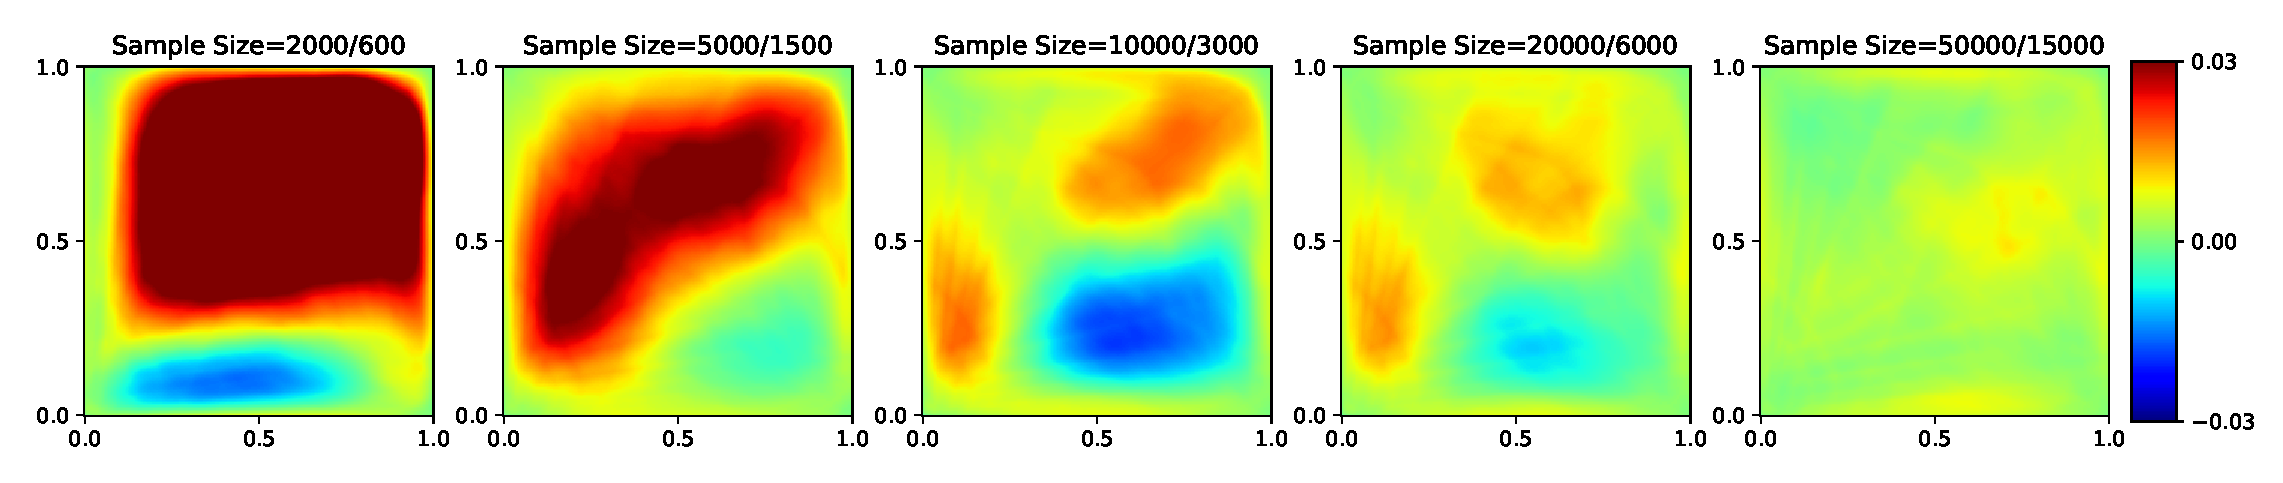
\includegraphics[width=\textwidth]{./figures2/func1_2d/HeatFig_n.eps}
    \caption{$($具有齐次边界条件的 Dirichlet 问题, $d=2)$。在不同样本量 $n$ 下，Deep Ritz 解 $u_{DRM}$ 与真解 $u_1(x)$ 之间的逐点差。} \label{fig:fig_n}
\end{figure}

\begin{figure}[htbp]
    \centering
    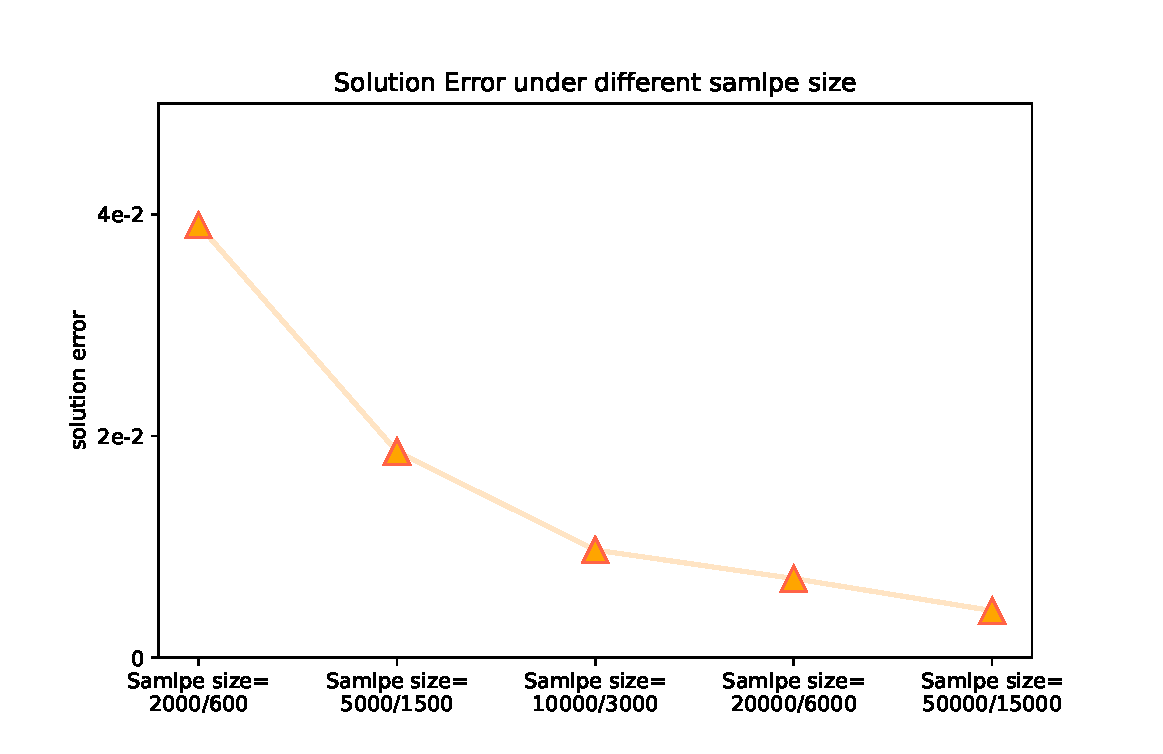
\includegraphics[width=0.5\textwidth]{./figures2/func1_2d/solution_err_under_diff_n.eps}
    \caption{$($具有齐次边界条件的 Dirichlet 问题, $d=2)$。在不同样本量 $n$ 下的 $L_2$ 解误差。} \label{fig:fig_n1}
\end{figure}

\textcolor{black}{首先，我们重点评估采样大小 $n$ 对解精度的影响。我们将网络参数设置为 $\mathcal{W} = 120$ 和 $\mathcal{D} = 4$，同时采用不同的采样大小来解决问题 \ref{eq:example1}。结果如图 \ref{fig:fig_n} 所示，且正如 图 \ref{fig:fig_n1} 中所预期的那样，较大的采样大小会导致较高的精度。这一观察结果与定理 \ref{mainthm:diri} 的结论一致。}

\textcolor{black}{值得注意的是，在上述数值实验中，我们在计算开始时仅对 $\{X_i\}_{i=1}^{n}$ 进行了一次采样。当 $n$ 较小时，算法表现不佳且收敛缓慢。为了同时提高算法的精度和效率，我们实施了一种在每个训练步或每几个训练步后对 $\{X_i\}_{i=1}^{n}$ 进行重采样的策略。这个过程类似于在无限样本集上的批量训练。通过采用这种方法，我们可以利用相对适度的计算资源有效地实现更大的 $n$，从而提高算法的泛化性能。我们的大量实验也证实了这种技术的有效性。除非另有说明，我们后续实验中提到的采样大小 $n$ 均指重采样的 $n$。}

\textcolor{black}{网络宽度 $\mathcal{W}$ 对该方法的影响如图 \ref{fig:fig_w} 和图 \ref{fig:fig_w1} 所示。我们在 $\mathcal{D} = 4$ 和 $n = 150000$ 的条件下进行了实验。实验结果表明，更宽的网络可以获得更高的精度并收敛得更快。这一发现与我们先前的结论一致。}

\begin{figure}[htbp]
    \centering
    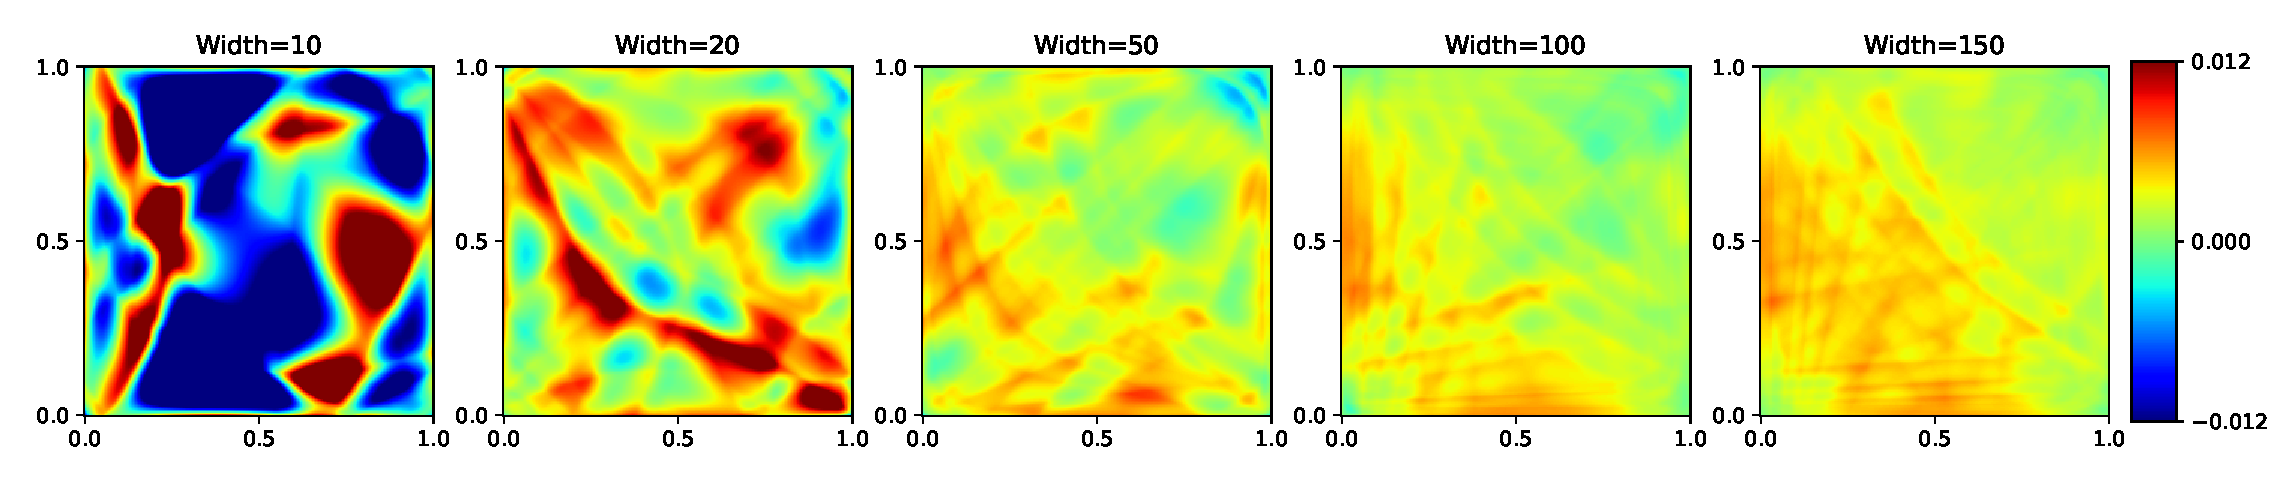
\includegraphics[width=\textwidth]{./figures2/func1_2d/HeatFig_w_5wstep.eps}
    \caption{$($具有齐次边界条件的 Dirichlet 问题， $d=2)$。在不同网络宽度 $\mathcal{W}$ 下，Deep Ritz 解 $u_{DRM}$ 与真解 $u_1(x)$ 之间的逐点差。} \label{fig:fig_w}
\end{figure}

\begin{figure}[htbp]
    \centering
    
    % --- 子图 1: L2 误差 ---
    % 建议使用 0.45\textwidth 到 0.48\textwidth
    \begin{subfigure}{0.48\textwidth}
        \centering
        % width=\linewidth 让图片自动充满子图容器(即上面的 0.48\textwidth)
        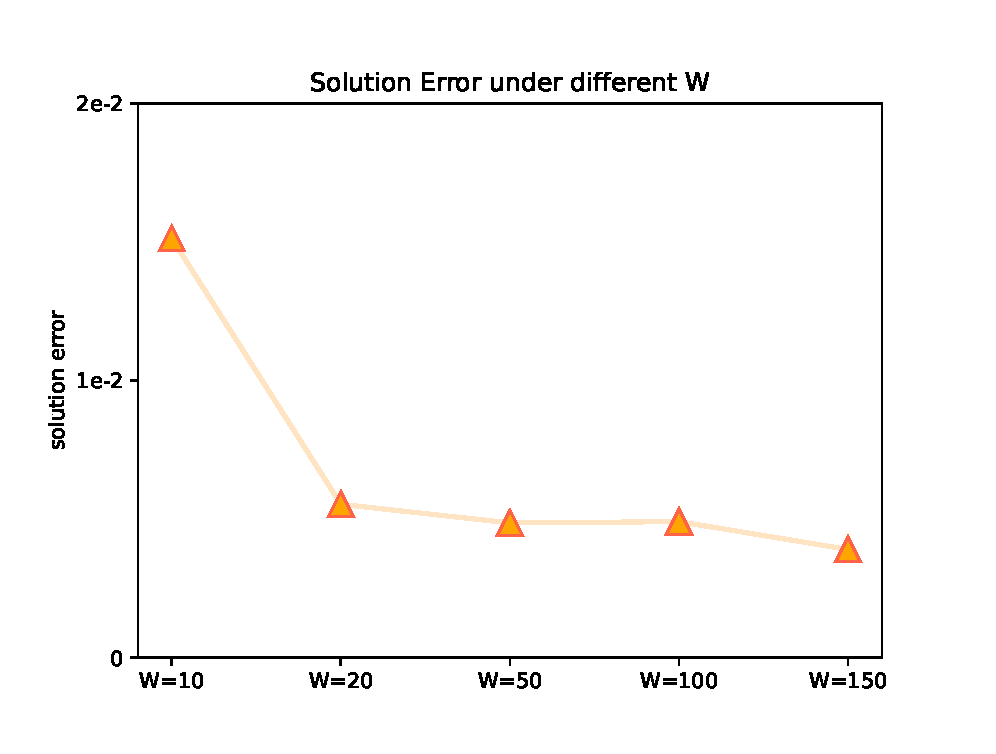
\includegraphics[width=\linewidth]{./figures2/func1_2d/solution_err_under_diff_w.eps}
        \caption{$L_2$ 解误差}
        \label{fig:l2_error_w}
    \end{subfigure}
    \hfill % 弹性间距，将两张图撑开
    % --- 子图 2: 训练误差 ---
    \begin{subfigure}{0.48\textwidth}
        \centering
        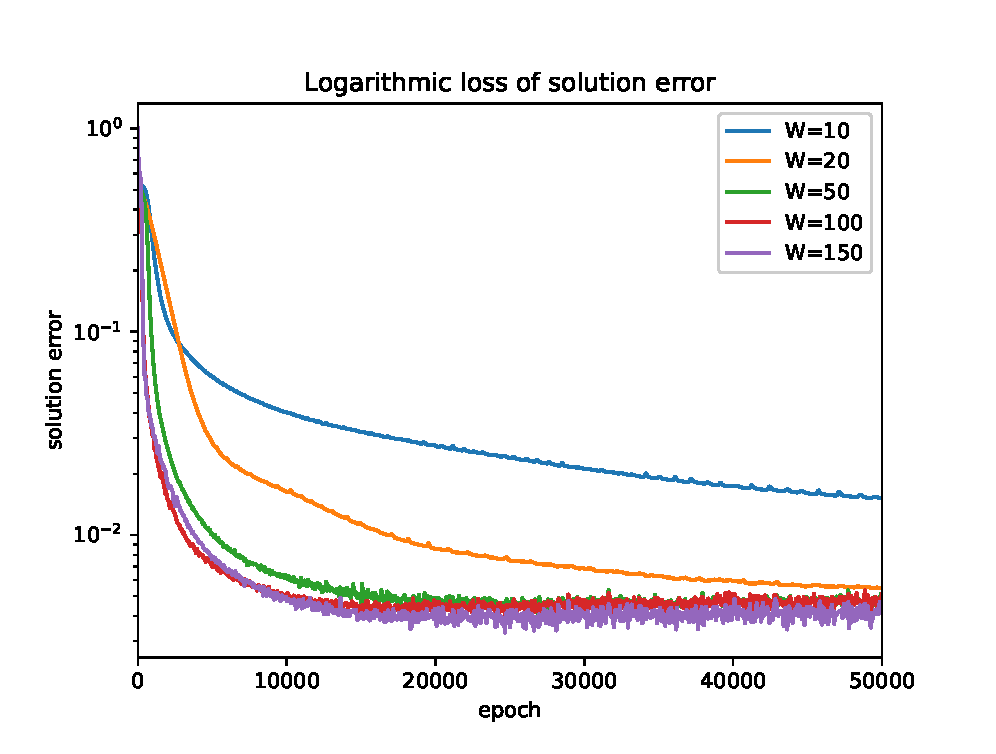
\includegraphics[width=\linewidth]{./figures2/func1_2d/Fig_w_5wstep.eps}
        \caption{训练过程中的误差}
        \label{fig:training_error_w}
    \end{subfigure}
    
    \caption{(具有齐次边界条件的 Dirichlet 问题， $d=2$)。Deep Ritz 方法在不同网络宽度 $\mathcal{W}$ 下的收敛性能。}
    \label{fig:fig_w1}
\end{figure}

\textcolor{black}{随后我们研究 $d=10$ 的情形。由于高维性以及 $S(x)$ 引入的非线性，求解该方程变得极具挑战性。传统的计算技术，如有限差分法 (FDM) 和有限元法 (FEM)，已被证明难以奏效。尽管面临这些挑战，Deep Ritz 方法依然有效，如图 \ref{fig:func1} 所示。我们在 $\Omega$ 的对角线上绘制了近似解和精确解，如图 \ref{fig:func1} (a) 所示。$L^{2}$ 误差随训练轮次的变化趋势如图 \ref{fig:func1} (b) 所示，损失函数如图 \ref{fig:func1} (c) 所示}

\textcolor{black}{该数值实验的参数配置如下：$\varepsilon=2000$，深度 $\mathcal{D}=4$，宽度 $\mathcal{W}=80$，样本量为 $200000$，边界样本量为 $80000$。我们采用 Adam 算法来最小化目标函数，初始学习率设定为 1.8e-3。采用了等间隔学习率衰减策略，其中学习率每隔 $5000$ 步衰减为原来的 $0.9$。}

\begin{figure}[htbp]
    \centering
    
    % --- 子图 1: 解的近似 ---
    \begin{subfigure}{0.32\textwidth}
        \centering
        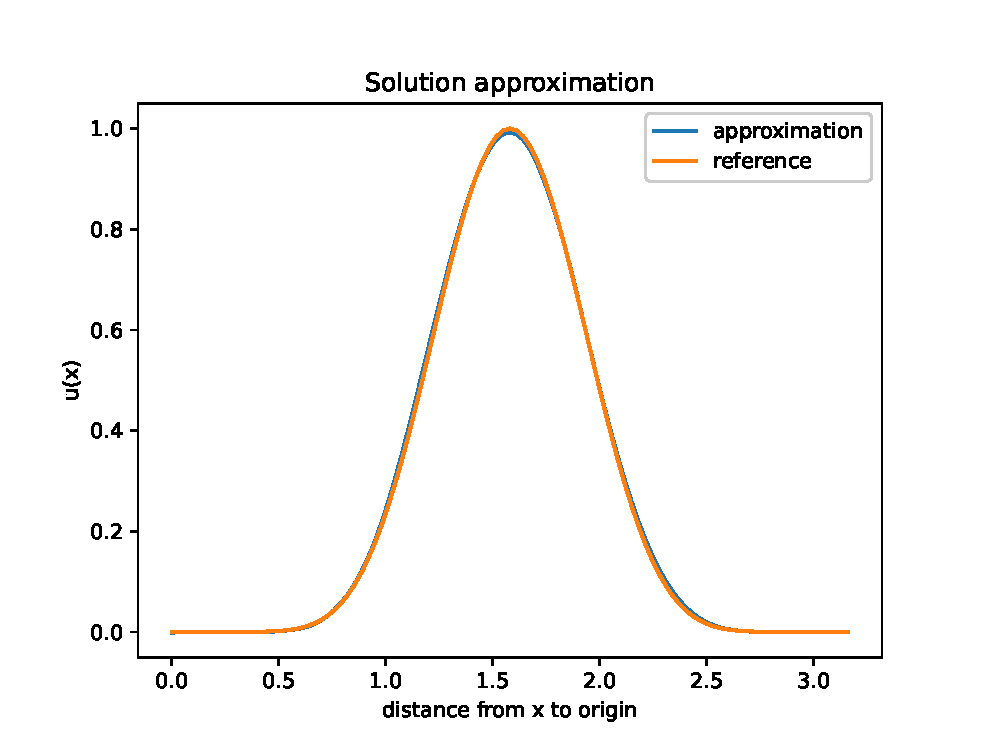
\includegraphics[width=\linewidth]{./figures2/func1/unn.eps}
        \caption{对角线上的解近似值}
        \label{fig:func1_approx}
    \end{subfigure}
    \hfill % 弹性间距
    % --- 子图 2: L2 误差 ---
    \begin{subfigure}{0.32\textwidth}
        \centering
        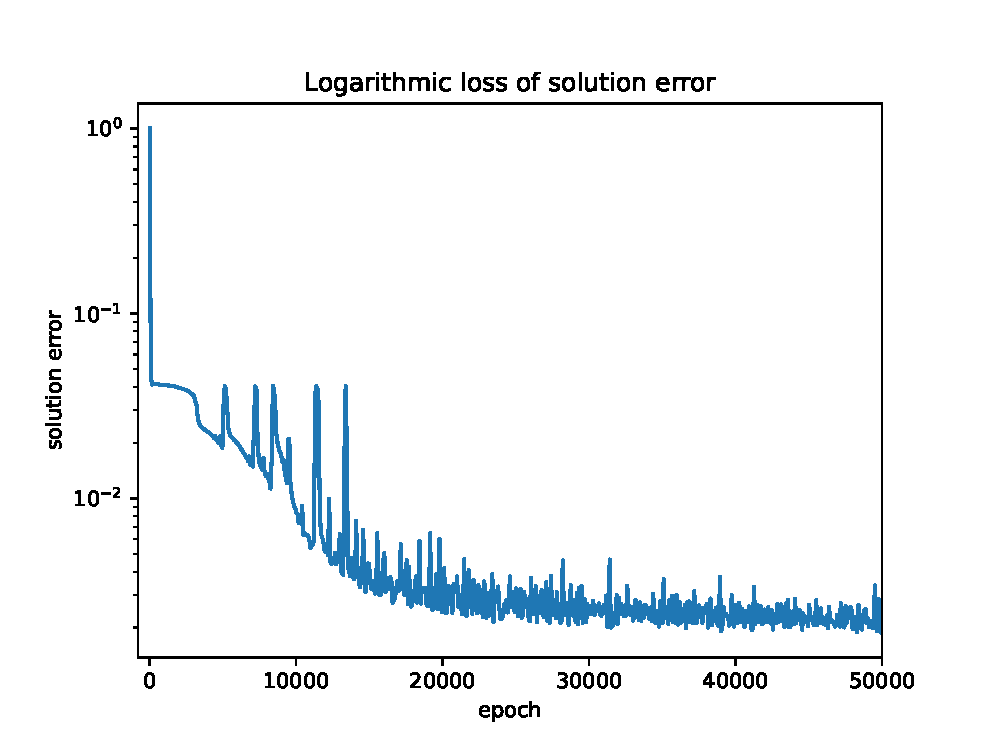
\includegraphics[width=\linewidth]{./figures2/func1/solution_err.eps}
        \caption{训练期间的 $L_2$ 误差}
        \label{fig:func1_err}
    \end{subfigure}
    \hfill % 弹性间距
    % --- 子图 3: 损失 ---
    \begin{subfigure}{0.32\textwidth}
        \centering
        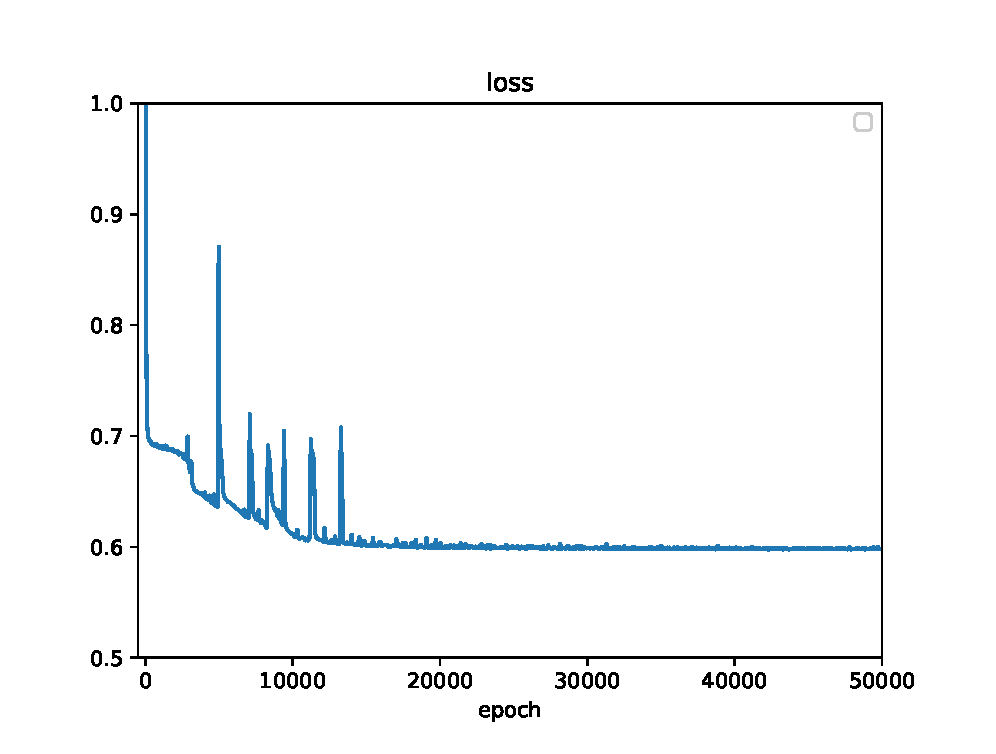
\includegraphics[width=\linewidth]{./figures2/func1/loss.eps}
        \caption{训练期间的损失函数}
        \label{fig:func1_loss}
    \end{subfigure}
    
    \caption{具有齐次边界条件的 Dirichlet 问题 ($d=10$)。由于无法直接可视化高维空间中的函数，此处展示立方体区域对角线上的值并与真实解对比。}
    \label{fig:func1}
\end{figure}


\subsection{具有非齐次边界条件的 Dirichlet 问题}
\textcolor{black}{为了说明我们理论的通用性，我们考虑以下非齐次 Dirichlet 问题。}
\begin{equation}\label{eq:example2}
\left\{\begin{aligned}
-\Delta u + S(u) & = g_2(x) & \text{在 } & \Omega \text{ 上},\\
Tu& = T g_2(x) & \text{在 } & \partial\Omega \text{ 上},\\
\end{aligned}\right.
\end{equation}

其中 $\Omega=[-1,1]^{10}$，并且
\begin{equation*}
g_2(x)=\left\{\begin{array}{lll}
\frac{2}{d} + S \left( \left(\frac{1}{d}\sum_{i=1}^{d}x_{i}\right)^{2} \right), & \left| \frac{1}{d}\sum_{i=1}^{d}x_{i} \right|> \sqrt{0.3},\\
S(0.3), & \left| \frac{1}{d}\sum_{i=1}^{d}x_{i} \right|\leq \sqrt{0.3},\\
\end{array}\right.
\end{equation*}
上述非齐次问题的解由下式给出：
\begin{equation*}
u_2(x)=\left\{\begin{array}{lll}
\left(\frac{1}{d}\sum_{i=1}^{d}x_{i}\right)^{2}, & \left| \frac{1}{d}\sum_{i=1}^{d}x_{i} \right|> \sqrt{0.3},\\
0.3, & \left| \frac{1}{d}\sum_{i=1}^{d}x_{i} \right|\leq \sqrt{0.3},\\
\end{array}\right.
\end{equation*}
与前一个方程相比，问题 \ref{eq:example2} 不仅是一个非齐次边界问题，而且涉及非光滑解。

\textcolor{black}{本次数值实验的参数配置如下：$\varepsilon=2000$，深度 $\mathcal{D}=4$，宽度 $\mathcal{W}=150$，样本量为 $150000$，边界样本量为 $40000$。其他参数与之前相同。如图 \ref{fig:func2} 所示，在此设置下，所提方法也能准确地逼近解。}

\begin{figure}[htbp]
    \centering
    
    % --- 第一张子图 ---
    % 设置宽度为 0.32 倍文本宽度，留出空隙给间距
    \begin{subfigure}{0.32\textwidth}
        \centering
        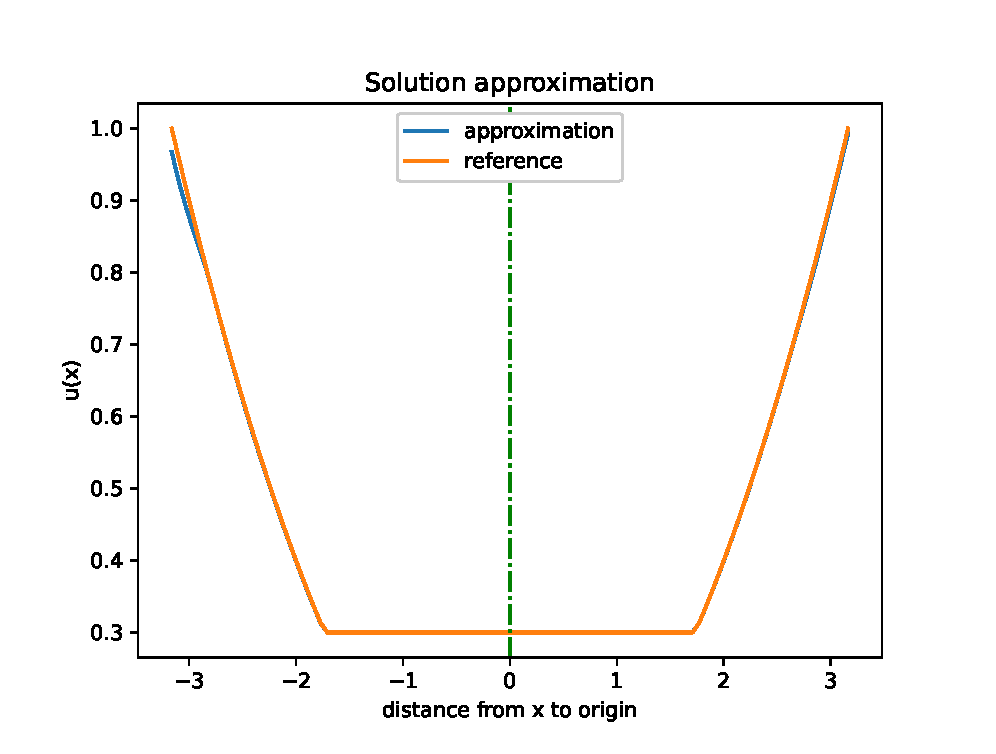
\includegraphics[width=\linewidth]{./figures2/func2/unn.eps}
        \caption{立方体区域对角线上的解逼近}
        \label{fig:func2_approx}
    \end{subfigure}
    \hfill % 弹性间距
    % --- 第二张子图 ---
    \begin{subfigure}{0.32\textwidth}
        \centering
        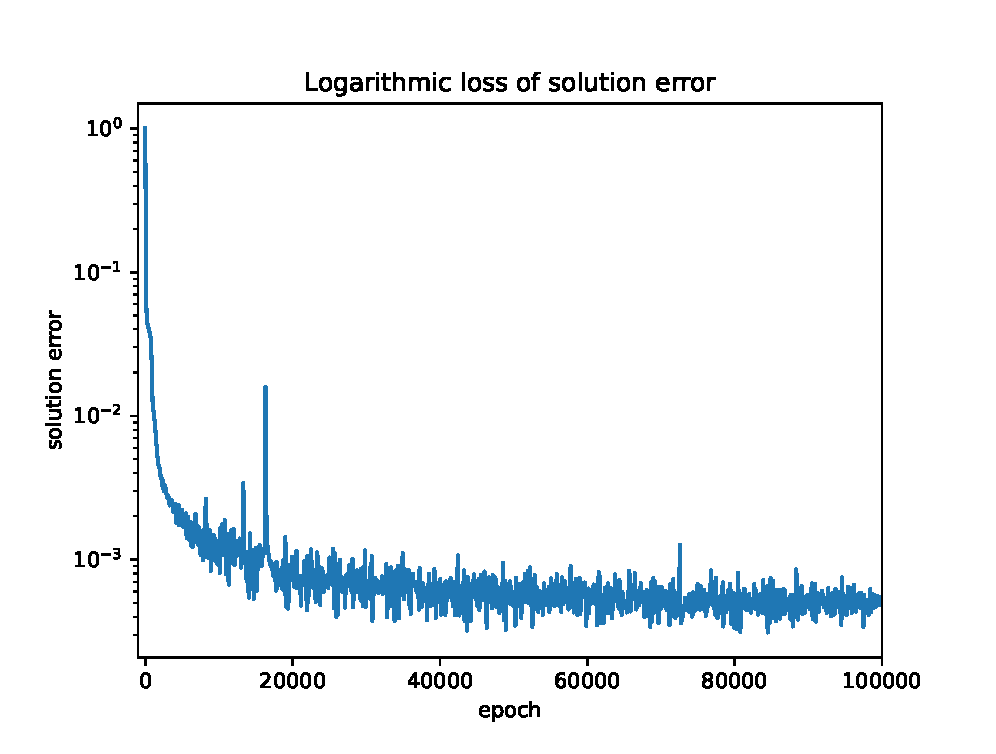
\includegraphics[width=\linewidth]{./figures2/func2/solution_err.eps}
        \caption{训练过程中的 $L_2$ 误差}
        \label{fig:func2_err}
    \end{subfigure}
    \hfill % 弹性间距
    % --- 第三张子图 ---
    \begin{subfigure}{0.32\textwidth}
        \centering
        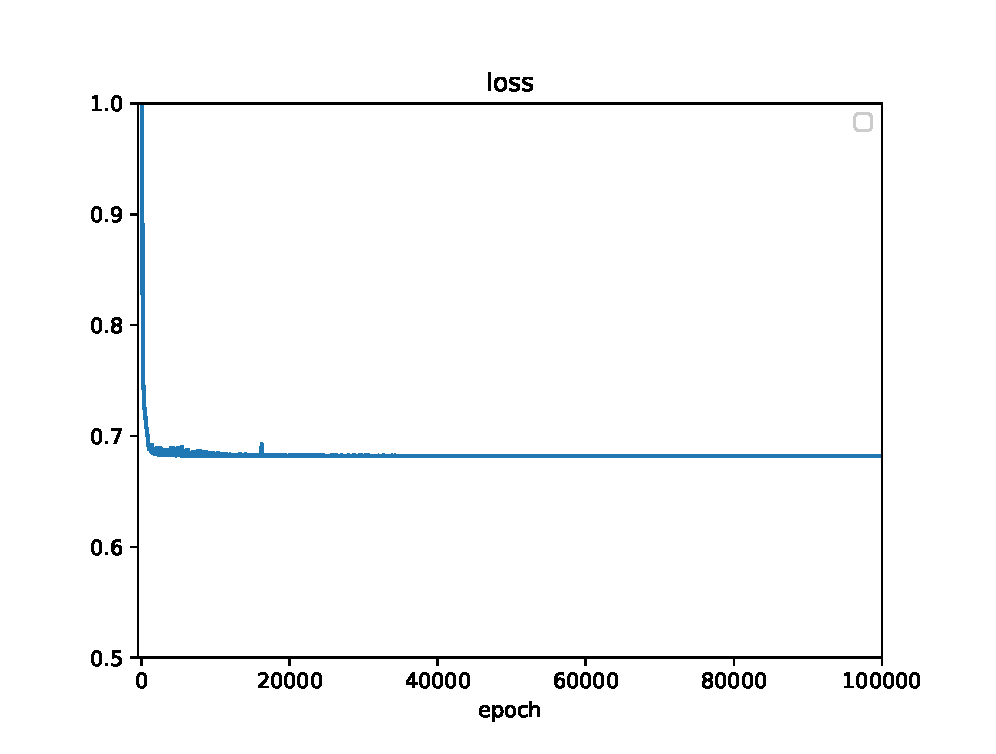
\includegraphics[width=\linewidth]{./figures2/func2/loss.eps}
        \caption{训练过程中的损失值}
        \label{fig:func2_loss}
    \end{subfigure}
    
    \caption{非齐次边界条件下的 Dirichlet 问题 ($d=10$)}
    \label{fig:func2}
\end{figure}



\section{讨论}\label{sec:dis}
在本文中，我们研究了利用具有 $\mathrm{ReLU}^2$ 激活函数的 ResNet 求解半线性椭圆问题。我们提出了一种基于惩罚变分形式的通用公式，用于计算半线性椭圆方程的解。随后，我们使用 Deep Ritz 方法对该惩罚变分形式进行求解。我们根据 $\mathrm{ReLU}^2$ ResNet 的深度 $\mathcal{D}$ 和宽度 $\mathcal{W}$ 以及训练样本数量 $n$，推导了估计解与真解之间误差的上界。我们的数值模拟结果证明了所提方法在克服维数灾难方面的有效性，并验证了我们的理论结果。

\section{附录}\label{sec:appd}
\textcolor{black}{在本附录中，我们给出了 4.3 节中引入的几个引理的完整证明。Deep Ritz 方法的统计误差分析遵循标准化流程，因此，正文中省略了这一部分。}

引理 \ref{lemma:staerr:Rad234} 的证明。
\begin{proof}\label{pf:lemma:staerr:Rad234}
我们将分两部分给出证明，每一部分都可以利用两个不同的事实单独获得。
第一个事实是 Rademacher 复杂度可以通过 Lipschitz 连续函数传递。这一事实使我们能够建立最后四个不等式：
\begin{lemma}\label{lemma:staerr:liprad}
假设 $\psi:\mathbb{R}^{d}\times\mathbb{R}\rightarrow\mathbb{R}$, $(x,y)\mapsto\psi(x,y)$ 对于所有 $x$ 在 $y$ 上是 $\ell$-Lipschitz 连续的。设 $\mathcal{N}$ 是 $\Omega$ 上的一类函数，且 $\psi\circ\mathcal{N}=\{\psi\circ u:x\mapsto\psi(x,u(x)) ,u\in\mathcal{N}\}$。那么
\begin{equation*}
\mathfrak{R}(\psi\circ\mathcal{N})\leq\ell \ \mathfrak{R}(\mathcal{N})
\end{equation*}
\end{lemma}
对于该陈述的推导，我们引用 \cite{ledoux2013probability} 中的推论 3.17。

显然，第 2、3、4 和 5 项的 Lipschitz 常数分别为 $2\|f\|_{\infty}$，$2K$，$2\varepsilon \mathcal{B}$ 和 $4\varepsilon \|h\|_{\infty}$。因此，可以以相同的方式直接得出它们的结论。

第一项需要特殊处理，因为 $\nabla$ 算子不是 Lipschitz 连续的。这一考虑直接遵循以下断言：
\par\noindent{\textbf{断言}：设 $u$ 是由深度为 $\mathcal{D}$ 且宽度为 $\mathcal{W}$ 的 $\mathrm{ReLU}^{2}$ 网络实现的函数。那么 $\|\nabla u\|_2^2$ 可以由深度为 $\mathcal{D}+3$ 且宽度为 $d\left(\mathcal{D}+2\right)\mathcal{W}$ 的 $\mathrm{ReLU}$-$\mathrm{ReLU}^{2}$ 网络实现。}

将 $\mathrm{ReLU}$ 和 $\mathrm{ReLU}^{2}$ 分别记为 $\sigma_1$ 和 $\sigma_2$。
只要我们证明每个偏导数 $D_iu(i=1,2,\cdots,d)$ 可以分别由 $\mathrm{ReLU}$-$\mathrm{ReLU}^{2}$ 网络实现，我们就可以轻松获得所需的网络，因为 $\|\nabla u\|_2^2=\sum_{i=1}^{d}\left|D_i u\right|^2$ 且平方函数可以通过 $x^2=\sigma_2(x)+\sigma_2(-x)$ 实现。
	
现在我们证明对于任何 $i=1,2,\cdots,d$，$D_iu$ 都可以由 $\mathrm{ReLU}$-$\mathrm{ReLU}^{2}$ 网络实现。我们将重点详细解释前两层，因为 $k\geq3$ 的层过程是类似的，并且可以通过归纳法推导。对于第一层，由于 $\sigma_2^{'}(x)=2\sigma_1(x)$，对于任何 $q=1,2\cdots,n_1$，我们有
\begin{equation*}
D_iu_q^{(1)}=D_i\sigma_2\left(\sum_{j=1}^{d}a_{qj}^{(1)}x_j+b_q^{(1)}\right)
=2\sigma_1\left(\sum_{j=1}^{d}a_{qj}^{(1)}x_j+b_q^{(1)}\right)\cdot a_{qi}^{(1)}
\end{equation*}
因此 $D_iu_q^{(1)}$ 可以由深度为 $2$ 宽度为 $1$ 的 $\mathrm{ReLU}$-$\mathrm{ReLU}^{2}$ 网络实现。对于第二层，
\begin{equation*}
D_iu_q^{(2)}=D_i\sigma_2\left(\sum_{j=1}^{n_1}a_{qj}^{(2)}u_j^{(1)}+b_q^{(2)}\right)
=2\sigma_1\left(\sum_{j=1}^{n_1}a_{qj}^{(2)}u_j^{(1)}+b_q^{(2)}\right)\cdot\sum_{j=1}^{n_1}a_{qj}^{(2)}D_iu_j^{(1)}.
\end{equation*}
由于 $\sigma_1\left(\sum_{j=1}^{n_1}a_{qj}^{(2)}u_j^{(1)}+b_q^{(2)}\right)$ 和 $\sum_{j=1}^{n_1}a_{qj}^{(2)}D_iu_j^{(1)}$ 可以分别由 $\mathrm{ReLU}-\mathrm{ReLU}^{2}$ 子网络实现，并且乘法也可以通过下式实现：
\begin{equation*}
\begin{split}
x\cdot y&=\frac{1}{4}\left[(x+y)^2-(x-y)^2\right]\\
&=\frac{1}{4}\left[\sigma_2(x+y)+\sigma_2(-x-y)-\sigma_2(x-y)-\sigma_2(-x+y)\right].
\end{split}
\end{equation*}
我们得出结论，$D_iu_q^{(2)}$ 可以由 $\mathrm{ReLU}$-$\mathrm{ReLU}^{2}$ 网络实现。我们有 $$\mathcal{D}\left(\sigma_1\left(\sum_{j=1}^{n_1}a_{qj}^{(2)}u_j^{(1)}+b_q^{(2)}\right)\right)=3, \mathcal{W}\left(\sigma_1\left(\sum_{j=1}^{n_1}a_{qj}^{(2)}u_j^{(1)}+b_q^{(2)}\right)\right)\leq\mathcal{W}$$ 以及 $$\mathcal{D}\left(\sum_{j=1}^{n_1}a_{qj}^{(2)}D_iu_j^{(1)}\right)=2, \mathcal{W}\left(\sum_{j=1}^{n_1}a_{qj}^{(2)}D_iu_j^{(1)}\right)\leq\mathcal{W}。$$ 因此 $\mathcal{D}\left(D_iu_q^{(2)}\right)=4,$ $\mathcal{W}\left(D_iu_q^{(2)}\right)\leq\max\{2\mathcal{W},4\}$。

现在我们对 $k\geq3$ 的层应用归纳法。对于第三层，
\begin{equation*}
D_iu_q^{(3)}=D_i\sigma_2\left(\sum_{j=1}^{n_2}a_{qj}^{(3)}u_j^{(2)}+b_q^{(3)}\right)
=2\sigma_1\left(\sum_{j=1}^{n_2}a_{qj}^{(3)}u_j^{(2)}+b_q^{(3)}\right)\cdot\sum_{j=1}^{n_2}a_{qj}^{(3)}D_iu_j^{(2)}.
\end{equation*}
由于
\begin{equation*}
\mathcal{D}\left(\sigma_1\left(\sum_{j=1}^{n_2}a_{qj}^{(3)}u_j^{(2)}+b_q^{(3)}\right)\right)=4, \mathcal{W}\left(\sigma_1\left(\sum_{j=1}^{n_2}a_{qj}^{(3)}u_j^{(2)}+b_q^{(3)}\right)\right)\leq\mathcal{W}
\end{equation*}
以及
\begin{equation*}
\mathcal{D}\left(\sum_{j=1}^{n_2}a_{qj}^{(3)}D_iu_j^{(2)}\right)=4, \mathcal{W}\left(\sum_{j=1}^{n_1}a_{qj}^{(3)}D_iu_j^{(2)}\right)\leq\max\{2\mathcal{W},4\mathcal{W}\}=4\mathcal{W},
\end{equation*}
我们得出结论，$D_iu_q^{(3)}$ 可以由 $\mathrm{ReLU}$-$\mathrm{ReLU}^{2}$ 网络实现，并且 $$\mathcal{D}\left(D_iu_q^{(3)}\right)=5, \mathcal{W}\left(D_iu_q^{(3)}\right)\leq\max\{5\mathcal{W},4\}=5\mathcal{W}。$$

我们假设 $D_iu_q^{(k)}(q=1,2,\cdots,n_k)$ 可以由 $\mathrm{ReLU}$-$\mathrm{ReLU}^{2}$ 网络实现，并且 $\mathcal{D}\left(D_iu_q^{(k)}\right)=k+2$, $\mathcal{W}\left(D_iu_q^{(3)}\right)\leq(k+2)\mathcal{W}$。对于第 $(k+1)$ 层，
\begin{align}
&D_iu_q^{(k+1)}=D_i\sigma_2\left(\sum_{j=1}^{n_k}a_{qj}^{(k+1)}u_j^{(k)}+b_q^{(k+1)}\right)\\
&=2\sigma_1\left(\sum_{j=1}^{n_k}a_{qj}^{(k+1)}u_j^{(k)}+b_q^{(k+1)}\right)\cdot\sum_{j=1}^{n_k}a_{qj}^{(k+1)}D_iu_j^{(k)}.
\end{align}
由于
\begin{equation*}
\begin{aligned}
\mathcal{D}\left(\sigma_1\left(\sum_{j=1}^{n_k}a_{qj}^{(k+1)}u_j^{(k)}+b_q^{(k+1)}\right)\right)&=k+2, \\
\mathcal{W}\left(\sigma_1\left(\sum_{j=1}^{n_k}a_{qj}^{(k+1)}u_j^{(k)}+b_q^{(k+1)}\right)\right)&\leq\mathcal{W},
\end{aligned}
\end{equation*}
以及
\begin{equation*}
\begin{aligned}
\mathcal{D}\left(\sum_{j=1}^{n_k}a_{qj}^{(k+1)}D_iu_j^{(k)}\right)&=k+2, \\ \mathcal{W}\left(\sum_{j=1}^{n_k}a_{qj}^{(k+1)}D_iu_j^{(k)}\right)&\leq\max\{(k+2)\mathcal{W},4\mathcal{W}\}=(k+2)\mathcal{W},
\end{aligned}
\end{equation*}
我们得出结论，$D_iu_q^{(k+1)}$ 可以由 $\mathrm{ReLU}$-$\mathrm{ReLU}^{2}$ 网络实现，并且 $\mathcal{D}\left(D_iu_q^{(k+1)}\right)=k+3$, $\mathcal{W}\left(D_iu_q^{(k+1)}\right)\leq\max\{(k+3)\mathcal{W},4\}=(k+3)\mathcal{W}$。
	
由此我们推导出 $D_iu=D_iu_1^{\mathcal{D}}$ 可以由 $\mathrm{ReLU}$-$\mathrm{ReLU}^{2}$ 网络实现，并且 $\mathcal{D}\left(D_iu\right)=\mathcal{D}+2$, $\mathcal{W}\left(D_iu\right)\leq\left(\mathcal{D}+2\right)\mathcal{W}$。最终，我们获得：
\begin{equation}\label{eq:N12}
    \mathcal{D}\left(\|\nabla u\|^2\right)=\mathcal{D}+3, \mathcal{W}\left(\|\nabla u\|^2\right)\leq d\left(\mathcal{D}+2\right)\mathcal{W}.
\end{equation}
\end{proof}

Proof of lemma \ref{lemma:staerr:Rad_cover}.
引理 \ref{lemma:staerr:Rad_cover} 的证明。
\begin{proof}
\label{pf:lemma:staerr:Rad_cover}
首先，我们介绍 Massart 有限类引理，其证明可以在 \cite{boucheron2013concentration} 中找到。
\begin{lemma}[Massart 有限类引理 \cite{boucheron2013concentration}]\label{Mfinite}
对于任意具有直径 $D=\sum_{v\in V}\|v\|_{2}$ 的有限集 $V\in\mathbb{R}^{n}$，有
\begin{equation*}
\mathbb{E}_{\sigma_{i}}\left[ \sup_{v\in V}\frac{1}{n}\left| \sum_{i}\sigma_{i}v_{i} \right| \right] \leq \frac{D}{n}\sqrt{2\log(2|V|)},
\end{equation*}
其中 $\{\sigma_{i}\}_{i=1}^{n}$ 是 Rademacher 变量，其定义与定义 \ref{def:staerr:radcom} 中相同。
\end{lemma}

令 $\varepsilon_{j}=2^{-k+1} B$。我们将 $\mathcal{F}_{k}$ 记为 $\mathcal{F}$ 的一个 $\varepsilon_{k}$-覆盖，且 $\left|\mathcal{F}_{k}\right|=\mathcal{C}\left(\varepsilon_{k}, \mathcal{F},\|\cdot\|_{\infty}\right) $。因此对于任意 $u \in \mathcal{F}$，存在 $u_{k} \in \mathcal{F}_{k}$ 使得 $\left\|u-u_{k}\right\|_{\infty} \leq \varepsilon_{k} $。设 $K$ 为一个稍后确定的正整数。我们有
\begin{equation*}
\begin{array}{rcl}
{}&{}&\mathbb{E}_{\left\{\sigma_{i}, Z_{i}\right\}_{i=1}^{n}}\left[\sup\limits_{u \in \mathcal{F}} \frac{1}{n}\left|\sum\limits_{i=1}^{n} \sigma_{i} u\left(Z_{i}\right)\right|\right]\\
{}&{}&{}\\
{}&=&\mathbb{E}_{\left\{\sigma_{i}, Z_{i}\right\}_{i=1}^{n}}\left[\sup\limits _{u \in \mathcal{F}} \frac{1}{n}\left|\sum\limits_{i=1}^{n} \sigma_{i}\left(u\left(Z_{i}\right)-u_{K}\left(Z_{i}\right)\right)\right.\right.\\
{}&{}&\left.\left.+\sum\limits_{j=1}^{K-1} \sum\limits_{i=1}^{n} \sigma_{i}\left(u_{j+1}\left(Z_{i}\right)-u_{j}\left(Z_{i}\right)\right)+\sum\limits_{i=1}^{n} \sigma_{i} u_{1}\left(Z_{i}\right)\right|\right]\\
{}&{}&{}\\
{}&\leq&\mathbb{E}_{\left\{\sigma_{i}, Z_{i}\right\}_{i=1}^{n}}\left[\sup\limits _{u \in \mathcal{F}} \frac{1}{n}\left|\sum\limits_{i=1}^{n} \sigma_{i}\left(u\left(Z_{i}\right)-u_{K}\left(Z_{i}\right)\right)\right|\right]\\
{}&{}&+\sum\limits_{j=1}^{K-1} \mathbb{E}_{\left\{\sigma_{i}, Z_{t}\right\}_{i=1}^{n}}\left[\sup\limits _{u \in \mathcal{F}} \frac{1}{n}\left|\sum\limits_{i=1}^{n} \sigma_{i}\left(u_{j+1}\left(Z_{i}\right)-u_{j}\left(Z_{i}\right)\right)\right|\right]\\
{}&{}&+\mathbb{E}_{\left\{\sigma_{i}, Z_{t}\right\}_{k=1}^{n}}\left[\sup\limits _{u \in \mathcal{F}} \frac{1}{n}\left|\sum\limits_{i=1}^{n} \sigma_{i} u_{1}\left(Z_{i}\right)\right|\right]
\end{array}
\end{equation*}
由于 $0 \in \mathcal{F}$，我们可以选择 $\mathcal{F}_{1}=\{0\}$ 来消去第三项。对于第一项，
\begin{equation*}
\begin{array}{rcl}
{}&{}&\mathbb{E}_{\left\{\sigma_{i}, Z_{i}\right\}_{t=1}^{n}}\left[\sup\limits _{u \in \mathcal{F}} \frac{1}{n}\left|\sum\limits_{i=1}^{n} \sigma_{i}\left(u\left(Z_{i}\right)-u_{K}\left(Z_{i}\right)\right)\right|\right]\\
{}&\leq&\mathbb{E}_{\left\{\sigma_{i}, Z_{i}\right\}_{i=1}^{n}}\left[\sup\limits _{u \in \mathcal{F}} \frac{1}{n} \sum\limits_{i=1}^{n}\left|\sigma_{i}\right|\left\|u-u_{K}\right\|_{\infty}\right] \leq \varepsilon_{K}
\end{array}
\end{equation*}
对于第二项，定义 $v_{i}^{j}=u_{j+1}\left(Z_{i}\right)-u_{j}\left(Z_{i}\right)$，并应用引理 \ref{Mfinite}，我们有
\begin{equation*}
\begin{aligned}
&\sum_{j=1}^{K-1} \mathbb{E}_{\{\sigma\}_{i=1}^{n}}\left[\sup _{u \in \mathcal{F}} \frac{1}{n}\left|\sum_{i=1}^{n} \sigma_{i}\left(u_{j+1}\left(Z_{i}\right)-u_{j}\left(Z_{i}\right)\right)\right|\right]                                              \\
=&\sum_{j=1}^{K-1} \mathbb{E}_{\left\{\sigma_{t}\right\}_{t=1}^{n}}\left[\sup _{v \in V_{j}} \frac{1}{n} \left| \sum_{i=1}^{n} \sigma_{i} v_{i}^{j}\right|\right] \leq \sum_{j=1}^{K-1} \frac{D_{j}}{n} \sqrt{2 \log \left(2\left|V_{j}\right|\right)}.
\end{aligned}
\end{equation*}
根据 $V_{j}$ 的定义，我们可知 $\left|V_{j}\right| \leq\left|\mathcal{F}_{j}\right|\left|\mathcal{F}_{j+1}\right| \leq\left|\mathcal{F}_{j+1}\right|^{2}$ 并且
\begin{equation*}
\begin{aligned}
\|V\|_{2} & =\left(\sum_{i=1}^{n}\left|u_{j+1}\left(Z_{i}\right)-u_{j}\left(Z_{i}\right)\right|^{2}\right)^{1 / 2} \leq \sqrt{n}\left\|u_{j+1}-u_{j}\right\|_{\infty}\\
&\leq \sqrt{n}\left\|u_{j+1}-u\right\|_{\infty}+\sqrt{n}\left\|u_{j}-u\right\|_{\infty}=\sqrt{n} \varepsilon_{j+1}+\sqrt{n} \varepsilon_{j}=3 \sqrt{n} \varepsilon_{j+1}.
\end{aligned}
\end{equation*}
因此
\begin{equation*}
\begin{aligned}
&\sum_{j=1}^{K-1} \mathbb{E}_{\left\{\sigma_{i}, Z_{t}\right\}_{t=1}^{n}}\left[\sup _{u \in \mathcal{F}} \frac{1}{n}\left|\sum_{i=1}^{n} \sigma_{i}\left(u_{j+1}\left(Z_{i}\right)-u_{j}\left(Z_{i}\right)\right)\right|\right] \\
&\leq \sum_{j=1}^{K-1} \frac{D_{j}}{n} \sqrt{2 \log \left(2\left|V_{j}\right|\right)} \leq \sum_{j=1}^{K-1} \frac{3 \varepsilon_{j+1}}{\sqrt{n}} \sqrt{2 \log \left(2\left|\mathcal{F}_{j+1}\right|^{2}\right)}
\end{aligned}
\end{equation*}
现在我们得到
\begin{equation*}
\begin{aligned}
&\mathbb{E}_{\left\{\sigma_{i}, Z_{i}\right\}_{i=1}^{n}}\left[\sup _{u \in \mathcal{F}} \frac{1}{n}\left|\sum_{i=1}^{n} \sigma_{i} u\left(Z_{i}\right)\right|\right] \leq \varepsilon_{K}+\sum_{j=1}^{K-1} \frac{6 \varepsilon_{j+2}}{\sqrt{n}} \sqrt{2 \log \left(2\left|\mathcal{F}_{j+1}\right|^{2}\right)} \\
&=\varepsilon_{K}+\frac{6}{\sqrt{n}} \sum_{j=1}^{K-1}\left(\varepsilon_{j+1}-\varepsilon_{j+2}\right) \sqrt{2 \log \left(2 \mathcal{C}\left(\varepsilon_{j+1}, \mathcal{F},\|\cdot\|_{\infty}\right)^{2}\right)}                                                                                                     \\
&\leq \varepsilon_{K}+\frac{6}{\sqrt{n}} \int_{\varepsilon_{K+1}}^{B / 2} \sqrt{2 \log \left(2 \mathcal{C}\left(\varepsilon, \mathcal{F},\|\cdot\|_{\infty}\right)^{2}\right)} d \varepsilon.
\end{aligned}
\end{equation*}
通过对于任意 $0<\delta<\frac{B}{2}$ 选择合适的 $K$ 使得 $\varepsilon_{K+2}<\delta \leq \varepsilon_{K+1}$，引理得证。
\end{proof}

引理 \ref{lemma:staerr:pdim} 的证明。
\begin{proof}
\label{pf:lemma:staerr:pdim}
证明概要如下：首先，引入 $VCdim$ 和伪打散 (pseudo-shattering) 作为 $Pdim$ 的下界；然后，通过 \cite{anthony2009neural} 中的一个引理估计多项式的 $VCdim$；基于上述结论，通过类似于 \cite{bartlett2019nearly} 中定理 6 的推导来完成证明。

以下是伪打散和 $VCdim$ 的定义。
\begin{definition}
令 $\mathcal{N}$ 为从 $X=\Omega(\partial \Omega)$ 到 $\{0,1\}$ 的函数集。假设 $S=\left\{x_{1}, x_{2}, \cdots, x_{n}\right\} \subset X$。如果对于任意 $b \in\{0,1\}^{n}$，存在一个 $u \in \mathcal{N}$ 满足
\begin{equation*}
u\left(x_{i}\right)=b_{i}, \quad i=1,2, \ldots, n,
\end{equation*}
则称 $S$ 被 $\mathcal{N}$ 打散 (shattered)。
\end{definition}

\begin{definition}
$\mathcal{N}$ 的 VC 维，记为 $\operatorname{VCdim}(\mathcal{N})$，定义为被 $\mathcal{N}$ 打散的所有集合中的最大基数。
\end{definition}

引入引理 \ref{lemma:covering_number} 来估计多项式的 $Pdim$。证明可以在 \cite{anthony2009neural} 的定理 8.3 中找到。
\begin{lemma}\label{lemma:covering_number}
令 $p_1,\cdots,p_m$ 为具有 $n$ 个变量且次数不超过 $d$ 的多项式。如果 $n\leq m$，则
\begin{equation*}
|\{(\operatorname{sign}(p_1(x)),\cdots,\operatorname{sign}(p_m(x))):x\in\mathbb{R}^n\}| \leq 2\left(\frac{2emd}{n}\right)^n.
\end{equation*}
\end{lemma}

该论证遵循 \cite{bartlett2019nearly} 中定理 6 的证明。此处陈述的结果比 \cite{bartlett2019nearly} 中的定理 6 略强，因为 $\mathrm{VCdim}(\operatorname{sign}(\mathcal{N}))\leq \mathrm{Pdim}(\mathcal{N})$。

我们考虑一个新的函数集：
\begin{equation*}
\mathcal{\widetilde{N}}=\{\widetilde{u}(x,y)=\operatorname{sign}(u(x)-y): u\in\mathcal{N}\},
\end{equation*}
显然 $\mathrm{Pdim}(\mathcal{N})\leq\mathrm{VCdim}(\mathcal{\widetilde{N}})$。我们现在界定 $\mathcal{\widetilde{N}}$ 的 VC 维。记 $\mathcal{M}$ 为实现 $\mathcal{N}$ 中函数的神经网络中的参数（权重和偏置）总数，我们的目标是针对所有 $\{x_i\}_{i=1}^{m}\subset X$ 和 $\{y_i\}_{i=1}^{m}\subset\mathbb{R}$，推导出
\begin{equation*}
K_{\{x_i\},\{y_i\}}(m):=|\{(\operatorname{sign}(u(x_{1}, a)-y_1), \ldots, \operatorname{sign}(u(x_{m}, a)-y_m)): a \in \mathbb{R}^{\mathcal{M}}\}|
\end{equation*}
的一致上界。实际上，$K_{\{x_i\},\{y_i\}}(m)$ 在所有 $\{x_i\}_{i=1}^{m}\subset X$ 和 $\{y_i\}_{i=1}^{m}\subset\mathbb{R}$ 上的最大值即为增长函数 $\mathcal{G}_{\mathcal{\widetilde{N}}}(m)$。

为了应用引理 \ref{lemma:covering_number}，我们将参数空间 $\mathbb{R}^{\mathcal{M}}$ 划分为若干子集，以确保在每个子集中 $u(x_i,a)-y_i$ 是关于 $a$ 的无断点多项式。事实上，我们的划分与 \cite{bartlett2019nearly} 中的划分相同。将该划分记为 $\{P_1,P_2,\cdots,P_N\}$，其中整数 $N$ 满足
\begin{equation} \label{pdimb1}
N\leq\prod_{i=1}^{\mathcal{D}-1}2\left(\frac{2emk_i(1+(i-1)2^{i-1})}{\mathcal{M}_i}\right)^{\mathcal{M}_i}
\end{equation}
其中 $k_i$ 和 $\mathcal{M}_i$ 分别表示实现 $\mathcal{N}$ 中函数的神经网络第 $i$ 层的单元数，以及截至第 $i$ 层（含）的所有层单元输入的参数总数。关于划分的构造，请参见 \cite{bartlett2019nearly}。显然我们有
\begin{equation} \label{pdimb2}
K_{\{x_i\},\{y_i\}}(m)\leq\sum_{i=1}^{N}|\{(\operatorname{sign}(u(x_{1}, a)-y_1), \cdots, \operatorname{sign}(u(x_{m}, a)-y_m)): a\in P_i\}|
\end{equation}
注意到 $u(x_i,a)-y_i$ 是关于 $a$ 的多项式，其次数与 $u(x_i,a)$ 的次数相同，即 $1 + (\mathcal{D}-1)2^{\mathcal{D}-1}$，如 \cite{bartlett2019nearly} 所示。因此，根据引理 \ref{lemma:covering_number}，我们有
\begin{align}
& |\{(\operatorname{sign}(u(x_{1}, a)-y_1), \cdots, \operatorname{sign}(u(x_{m}, a)-y_m)): a\in P_i\}|\nonumber                          \\
& \leq2\left(\frac{2em(1+(\mathcal{D}-1)2^{\mathcal{D}-1})}{\mathcal{M}_{\mathcal{D}}}\right)^{\mathcal{M}_{\mathcal{D}}}\label{pdimb3}.
\end{align}
结合 (Eq.~\eqref{pdimb1})，(Eq.~\eqref{pdimb2})，(Eq.~\eqref{pdimb3}) 可得
\begin{equation*}
K_{\{x_i\},\{y_i\}}(m)\leq\prod_{i=1}^{\mathcal{D}}2\left(\frac{2emk_i(1+(i-1)2^{i-1})}{\mathcal{M}_i}\right)^{\mathcal{M}_i}.
\end{equation*}
随之我们有
\begin{equation*}
\mathcal{G}_{\mathcal{\widetilde{N}}}(m)\leq\prod_{i=1}^{\mathcal{D}}2\left(\frac{2emk_i(1+(i-1)2^{i-1})}{\mathcal{M}_i}\right)^{\mathcal{M}_i},
\end{equation*}
因为 $K_{\{x_i\},\{y_i\}}(m)$ 在所有 $\{x_i\}_{i=1}^{m}\subset X$ 和 $\{y_i\}_{i=1}^{m}\subset\mathbb{R}$ 上的最大值是增长函数 $\mathcal{G}_{\mathcal{\widetilde{N}}}(m)$。使用与 \cite{bartlett2019nearly} 中定理 6 证明相同的代数推导，我们获得
\begin{equation*}
\mathrm{Pdim}(\mathcal{N})\leq C\left(\mathcal{D}^2\mathcal{W}^2 \log \mathcal{U}+\mathcal{D}^3\mathcal{W}^2\right)
\leq C\left(\mathcal{D}^2\mathcal{W}^2\left( \mathcal{D}+\log \mathcal{W}\right)\right)
\end{equation*}
其中 $\mathcal{U}$ 指的是实现 $\mathcal{N}$ 中函数的神经网络的单元数。
\end{proof}
%%%%==========================================================%%%
